\documentclass[12pt, a4paper]{article}

%%%%%%%%%%%%%%%%%%%%%%%%%%%%%%%%%%%%%%%%%%%%%%%%%%%%%%%%%%%%%%%%%%%%%%%%%%%%%%%%%%%%%%%%%%%%%%%%%%%%%%%%%%%%%%%%%%%%%%%%%%%%%%%%%%%%%%%%%%%%%%%%%%%%%%%%%%%%%%%%%%%%%%%%%%%%%%%%%%%%%%%%%%%%%%%%%%%%%%%%%%%%%%%%%%%%%%%%%%%%%%%%%%%%%%%%%%%%%%%%%%%%%%%%%%%%
\usepackage{amsmath}
\usepackage[colon]{natbib}
\usepackage[pdftex]{color, graphicx}
%\usepackage{hyperref}
%\usepackage{pause}
\usepackage{tabularx}
\usepackage{multicol}
\usepackage{bbm}
% \usepackage{bbold}
%\usepackage{pp4link}
%\usepackage{mpmulti}
\usepackage{graphicx}
% \usepackage{subfigure}
\usepackage{caption}
\usepackage{subcaption}
\usepackage{amsmath, amsthm, amssymb}
\usepackage{bbm}
%\usepackage{ulem}
\usepackage{pdfpages}
\usepackage{pgffor}
\usepackage{pdflscape}
\usepackage{tikz}
\usepackage{ctable}
\newtheorem{defin}{Definition}
\newtheorem{prop}{Proposition}
\usepackage{verbatim}
\usepackage{booktabs}
\usepackage{longtable}
\usepackage{rotating}
\usepackage{pdflscape}
\usepackage{geometry}
\usepackage[capposition=top]{floatrow}
\usepackage{rotating,geometry,setspace}
\usepackage{epstopdf}
\usepackage{pdflscape}\newcommand{\csm}[1]{{\color{green}[#1]}}
\usepackage{float}
\usepackage{subfloat}
% \usepackage[labelformat=simple]{subfig}
\usepackage{adjustbox}
\usepackage{ragged2e}
\usepackage{comment}
\usepackage{sectsty}
\usepackage{placeins} 
\usepackage{float}

\usepackage{subfig}
\usepackage{graphicx}
\usepackage{caption}
\usepackage{subcaption}
\usepackage{algorithm}
\usepackage{algpseudocode}

\usepackage{bigdelim}
%\usepackage{babel}
% \usepackage{mathptmx}
\usepackage{mathrsfs}
\usepackage{caption}
\usepackage[toc,page]{appendix}
\usepackage{stackengine}
\usepackage{multirow}
\usepackage[flushleft]{threeparttable}
%\usepackage{soul}
%\usepackage{cancel}
\usepackage[colorlinks=true,
            linkcolor=blue,
            urlcolor=blue,
            citecolor=blue]{hyperref}
\usepackage[T1]{fontenc}
\usepackage[utf8]{inputenc}
%\fontfamily{cmr}\selectfont

%\renewcommand{\familydefault}{\sfdefault}
%\usepackage{helvet}
%\usepackage{lmodern}
%\fontfamily{lmss}\selectfont

\usetikzlibrary{decorations.pathmorphing}
\usetikzlibrary{arrows, patterns,snakes}
\usepackage{gensymb}
\usepackage{dsfont}

\usepackage{pgf, tikz, tkz-tab}
\usepackage{subcaption, caption}
\usepackage{CJKutf8}
\usetikzlibrary{calc, intersections, through, backgrounds}
%\usepackage{amsmath, amsfonts, fancyhdr, amssymb, subcaption, caption}
%\usepackage[mathscr]{euscript}
%\usepackage{pgfplots}
\usetikzlibrary{patterns}
\usetikzlibrary{decorations.pathreplacing}
\usepackage[makeroom]{cancel}
\usepackage{bbm}
\usepackage{amsmath, amsthm, amssymb}

\usepackage{dcolumn}
\usepackage{colortbl} % To color table cells and rows
\newcommand{\sym}[1]{\rlap{#1}}
\newcommand{\labelthistable}{}
\justifying

%\usepackage{tikz}



\usepackage{color}
%\usepackage[usenames,dvipsnames,svgnames,table]{xcolor}
\usepackage[colorlinks=true,
            linkcolor=red,
            urlcolor=blue,
            citecolor=blue]{hyperref}

\setcounter{MaxMatrixCols}{10}

%\geometry{verbose,tmargin=1in,bmargin=1in,lmargin=1in,rmargin=1in}
\geometry{letterpaper,tmargin=1in,bmargin=1in,lmargin=0.95in,rmargin=0.95in}
\linespread{1.3} 
%\doublespace
\setlength{\footnotesep}{0.7\baselineskip}
\newtheorem{result}{Proposition}
\newtheorem{claim}{Claim}
\newtheorem{assumption}{Assumption}
\renewcommand{\qed}{\quad \rule{1.8mm}{1.8mm}}
\def\sym#1{\ifmmode^{#1}\else\(^{#1}\)\fi}
%\input{tcilatex}

\usepackage[utf8]{inputenc}
\usepackage{newunicodechar}
\usepackage[normalem]{ulem}
%\newunicodechar{¥}{\textyen}
\DeclareTextCommandDefault{\textyen}{%
  \vphantom{Y}%
  {\ooalign{Y\cr\hidewidth\yenbars\hidewidth\cr}}%
}

\newcommand{\yenbars}{%\textyen
  \vbox{
     \hrule height.1ex width.4em
     \kern.15ex
     \hrule height.1ex width.4em
     \kern.3ex
  }%
}

\let\oldemptyset\emptyset
\let\emptyset\varnothing
\newcommand\hcancel[2][black]{\setbox0=\hbox{$#2$}%
\rlap{\raisebox{.45\ht0}{\textcolor{#1}{\rule{\wd0}{1pt}}}}#2} 

\usepackage{etoc}

\newcommand{\comm}[1]{{\color{red}[#1]}}
\newcommand\barbelow[1]{\stackunder[1.2pt]{$#1$}{\rule{.8ex}{.075ex}}}
\newcommand{\st}{\sout} 

\definecolor{myorange}{RGB}{191,87,0}
\newcommand{\pjb}{\textcolor{red}} 
\newcommand{\tx}{\textcolor{blue}} 
 \usepackage{dsfont}

\setlength{\parskip}{1em}
\setlength{\parindent}{0em}

\begin{document}

\title{{\vspace{-2cm} \textbf{{Heat, Health, and Harm: The Impact of Extreme Temperatures on Suicide}}}

\author{\normalsize{Yegor Baranovski}
\thanks{Baranovski: 
Honors Economics Undergraduate Thesis, UW-Madison, yegorbar01@gmail.com. Special thanks to my advisor Professor Ashley Swanson for overseeing my work and putting up with me, along with the countless people I complained and vented to.}   } }

%\date{\today}
\vspace{-0.0in}
\date{\normalsize{ \vspace{0.0in} \today  \\ \vspace{0.0in} 
}
} 
% \vspace{-2cm}
\maketitle

\thispagestyle{empty}%
\vspace{-0.5cm} 

\begin{abstract}
\noindent  

Climate change poses well-established risks to physical health, but little is known about its effects on mental health.  I study the relationship between extreme temperature exposure during summer months and suicide risk in the United States from 1989 to 2019 using comprehensive county-level data on all deaths by suicide and high-resolution satellite-based temperature measurements. I identify the causal effects of extreme heat on suicide by relating year-over-year fluctuations in county-level summer monthly average temperatures to fluctuations in suicide rates. I compare these effects across urban and rural areas and various population subgroups. My results indicate that an increase of one defined extreme heat day in a summer month leads to approximately 0.091 additional suicide deaths per million residents for summer months, with effects concentrated among men and working-age adults, demographic groups already characterized by elevated baseline suicide risk. This paper provides large-scale empirical evidence that climate-related extreme heat significantly elevates suicide risk, underscoring the urgent need for targeted public health interventions to mitigate climate-induced mental health burdens.



\end{abstract} 
\newpage
\tableofcontents
\newpage

\vspace{0.0in}
% \begin{description}
% \item[Keywords:] Central negotiation, Insurance expansion, Innovative Drugs, China
% \item[JEL] Classification Codes: L91, R13, R21\newpage {}
% \end{description}

\pagenumbering{arabic}
\thispagestyle{empty}\setcounter{page}{1}
\section{Introduction}
\subsection{Motivation}
Mental illness represents an enormous and expanding global health challenge, both economically and socially. In the United States, approximately 49,450 individuals die by suicide each year, contributing to the nearly 727,000 suicide deaths recorded worldwide annually \cite{usSuicideStat}, \cite{whoSuicideStat}. The prevalence of mental health issues is also high, with 23.1\% of U.S. adults reporting a diagnosable mental, emotional, or behavioral disorder as of 2022 \cite{usMentalStat}. Financially, mental disorders impose substantial direct and indirect costs. Total direct societal burden was estimated to be \$280 billion and is expected to rise, making mental illness the costliest medical category in the country \cite{MHCost}. When considering indirect costs, including reduced productivity, lost wages, disability, and mortality, the total societal impact approaches \$450 billion annually in the U.S. and around \$2.5 trillion globally, figures projected to double by 2030 \cite{futureMHCost}. Beyond these economic impacts, mental health disorders also exacerbate physical health conditions, significantly increasing the overall health burden \cite{noHealthwoMH}.

Climate conditions are increasingly recognized as influential on various aspects of human health, impacting outcomes ranging from vector-borne disease prevalence to rates of cardiovascular incidents \cite{Patz2014}, \cite{Watts2015}. These health outcomes can be driven by direct physical stress (such as heatstroke or cyclone-related injuries), shifts in disease ecology (such as influenza or malaria dynamics), or socioeconomic disruptions such as drought-related famine \cite{Watts2015}. Additionally, studies indicate that higher temperatures may increase interpersonal conflicts and violence, potentially through economic stress or physiological responses that heighten aggression \cite{Hsiang2013}.

Despite extensive research into physical health impacts, the connection between climate factors and mental health, specifically suicide rates, has received limited quantitative analysis \cite{Berry2010}, \cite{burke2018}. Understanding this link is critical, given that suicide deaths globally exceed those caused by interpersonal and group violence combined \cite{Lim2013}, rank among the top causes of death worldwide, and represent a significant portion of lost life-years, particularly in wealthier nations \cite{Lozano2013}. In the United States specifically, suicide is one of the leading causes of death among individuals aged 10–54 \cite{cdcWisqars} and uniquely remains stable or increasing, unlike other major causes of death which are generally declining \cite{Swanson2015}. Consequently, even modest climate-related increases in suicide rates could significantly elevate global mental health burdens, particularly in developed regions already experiencing high or rising suicide incidence.

\subsection{Contribution}
This paper contributes a unique approach in quantifying the relationship between suicide risk and climate change. Specifically, I analyze the effects of extreme and abnormal heat on mental health-related mortality, using a granular and wide-ranging dataset to compare impacts between urban and rural areas across multiple demographic subgroups. My approach offers four distinct advantages.

First, to more comprehensively capture mental health-related mortality, I define mental health-related deaths to include not only suicides but also deaths classified as injuries of undetermined intent and certain types of accidental deaths (such as poisoning, firearm, train, and drowning incidents), defined further in Section 2.2. This broader definition addresses the known problem of misclassification in mortality data \cite{MHClassification}, where some suicides may be recorded as accidents due to reporting practices or legal ambiguity. By including categories plausibly linked to underlying mental health crises, this approach provides a more complete measure of the population-level impact of extreme heat on mental health, improving power. I use suicide risk and mental health mortality in this paper interchangeably.

\begin{figure}[H]
    \centering
    \caption{Average Monthly Suicide Rate(Deaths per Million) by County}
    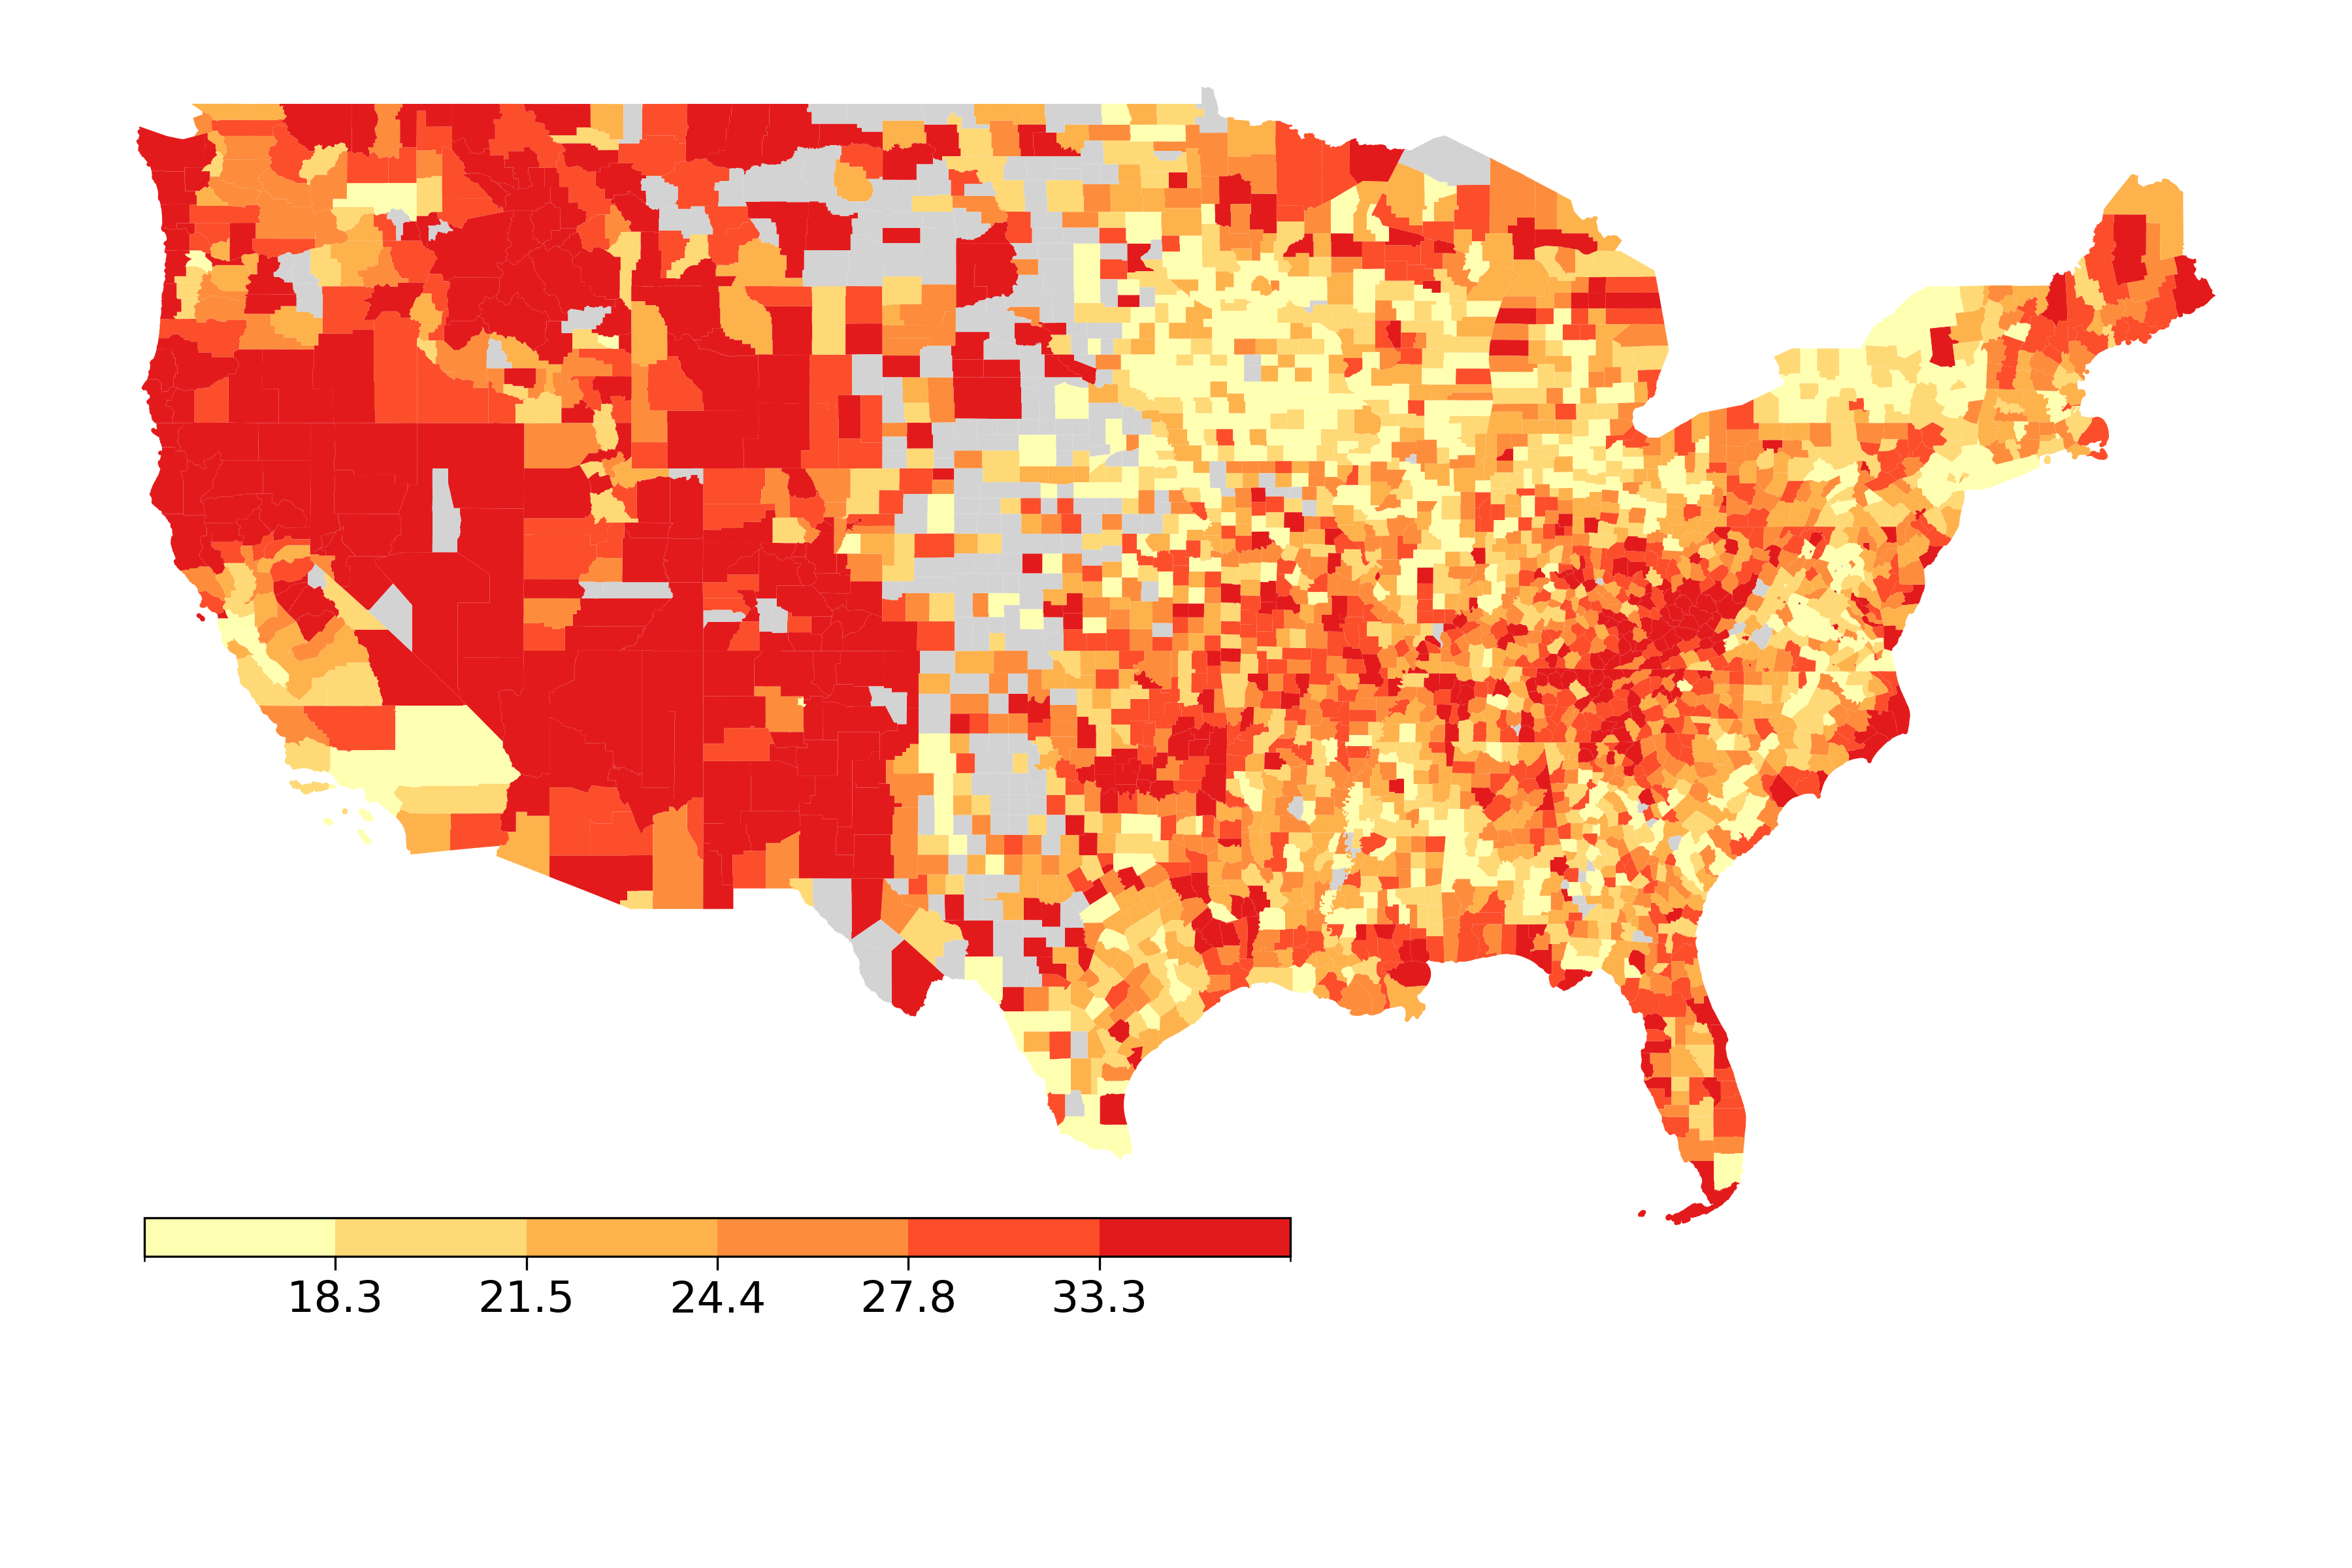
\includegraphics[width=0.8\textwidth]{suicide map.png}
    \label{fig:suicide_map}
\end{figure}

Second, I define extreme heat exposure using both relative and absolute threshold criteria, rather than relying solely on simple temperature averages. Specifically, I calculate extreme heat days (EHDs) as the number of days in a month where the daily mean temperature exceeds either the 85th percentile of the 30-year historical monthly distribution for a given county or a daily mean temperature threshold of $30\degree$C. This dual-definition approach contextualizes "extreme" relative to local climatological norms and human acclimation \cite{periard2016} while also accounting for objective human physiological tolerance levels, enabling more meaningful comparisons across regions and over time, and better capturing the types of heat events most relevant to health outcomes.

\begin{figure}[H]
    \centering
    \caption{Average Summer Percentile Thresholds(°C) by County}
    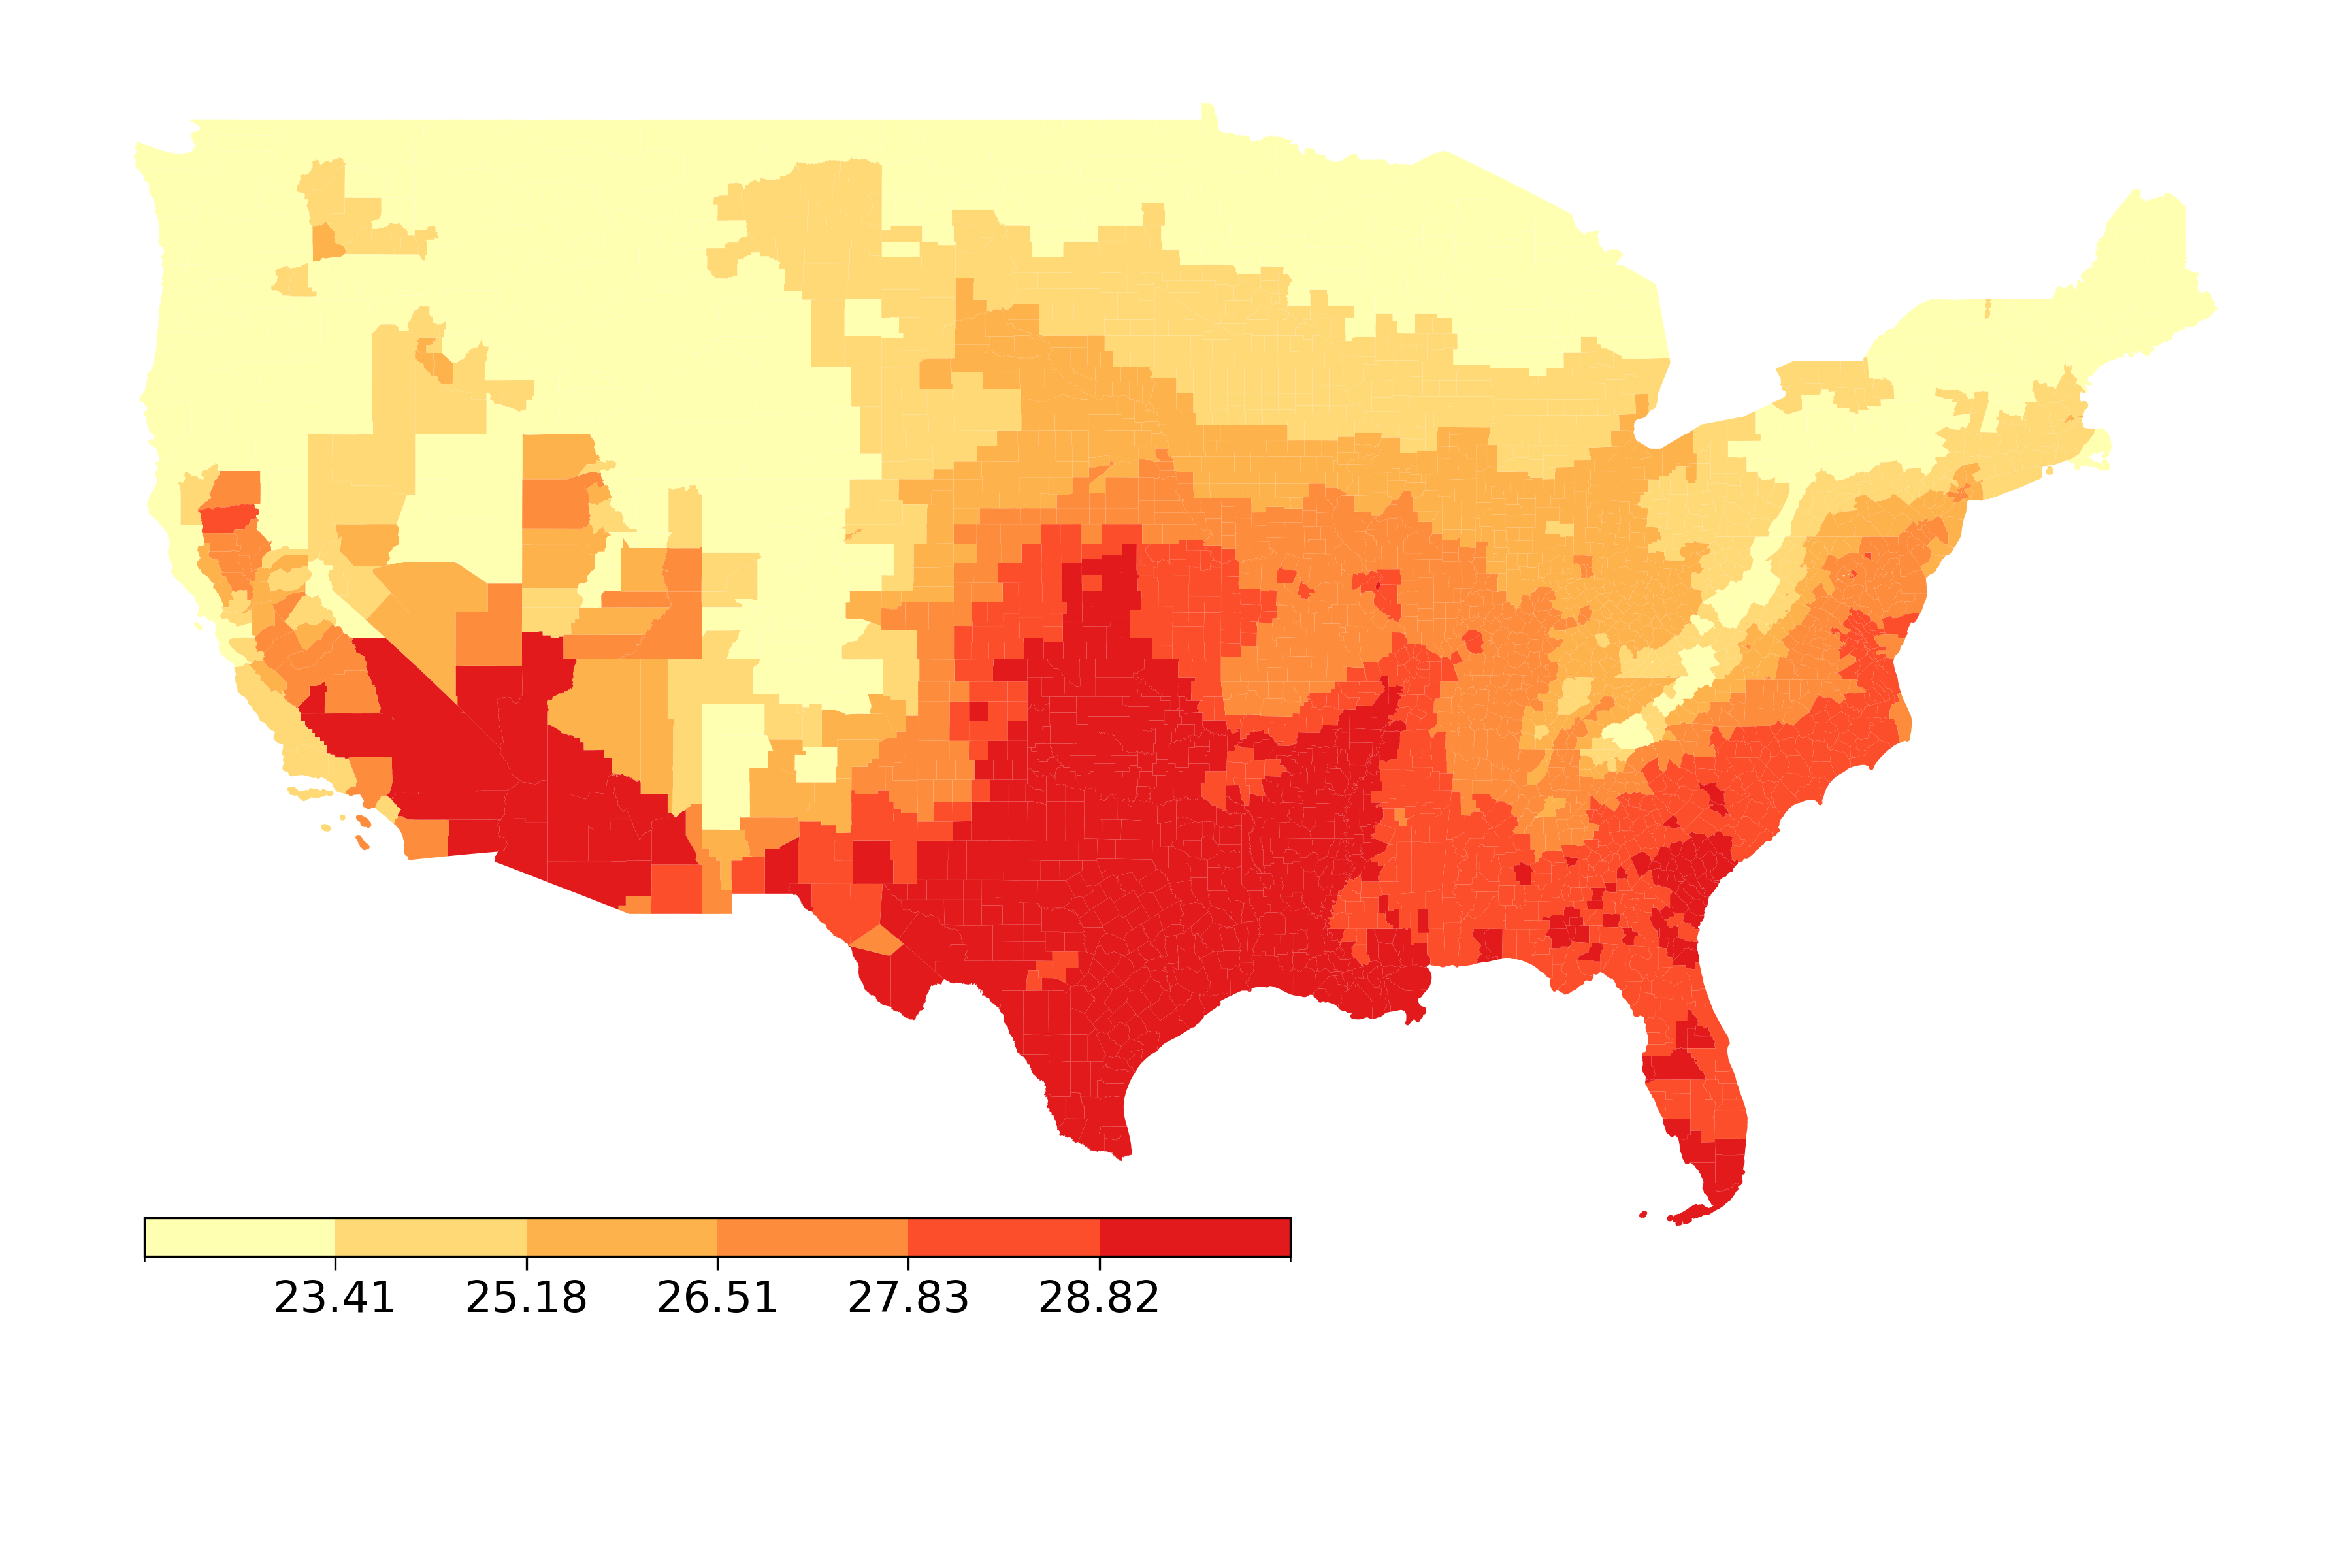
\includegraphics[width=0.8\textwidth]{thresholds.png}
    \label{fig:thresholds_map}
\end{figure}

Third, the estimated effects presented in this paper represent a lower bound on the true impact of temperature on mental health-related mortality. By defining extreme heat days using relatively high thresholds, either exceeding the 85th percentile of historical daily temperatures or surpassing $30\degree$C, this approach focuses on only the most severe temperature exposures. However, milder but still abnormal heat events, as well as cumulative heat stress from sustained periods of moderately high temperatures, may also contribute to adverse mental health outcomes \cite{HandHWHO}. As such, the full burden of heat on mental health could be even larger than what is captured by the estimates reported here.

\begin{figure}[H]
    \centering
    % First subfigure
    \begin{subfigure}[b]{0.48\textwidth}
        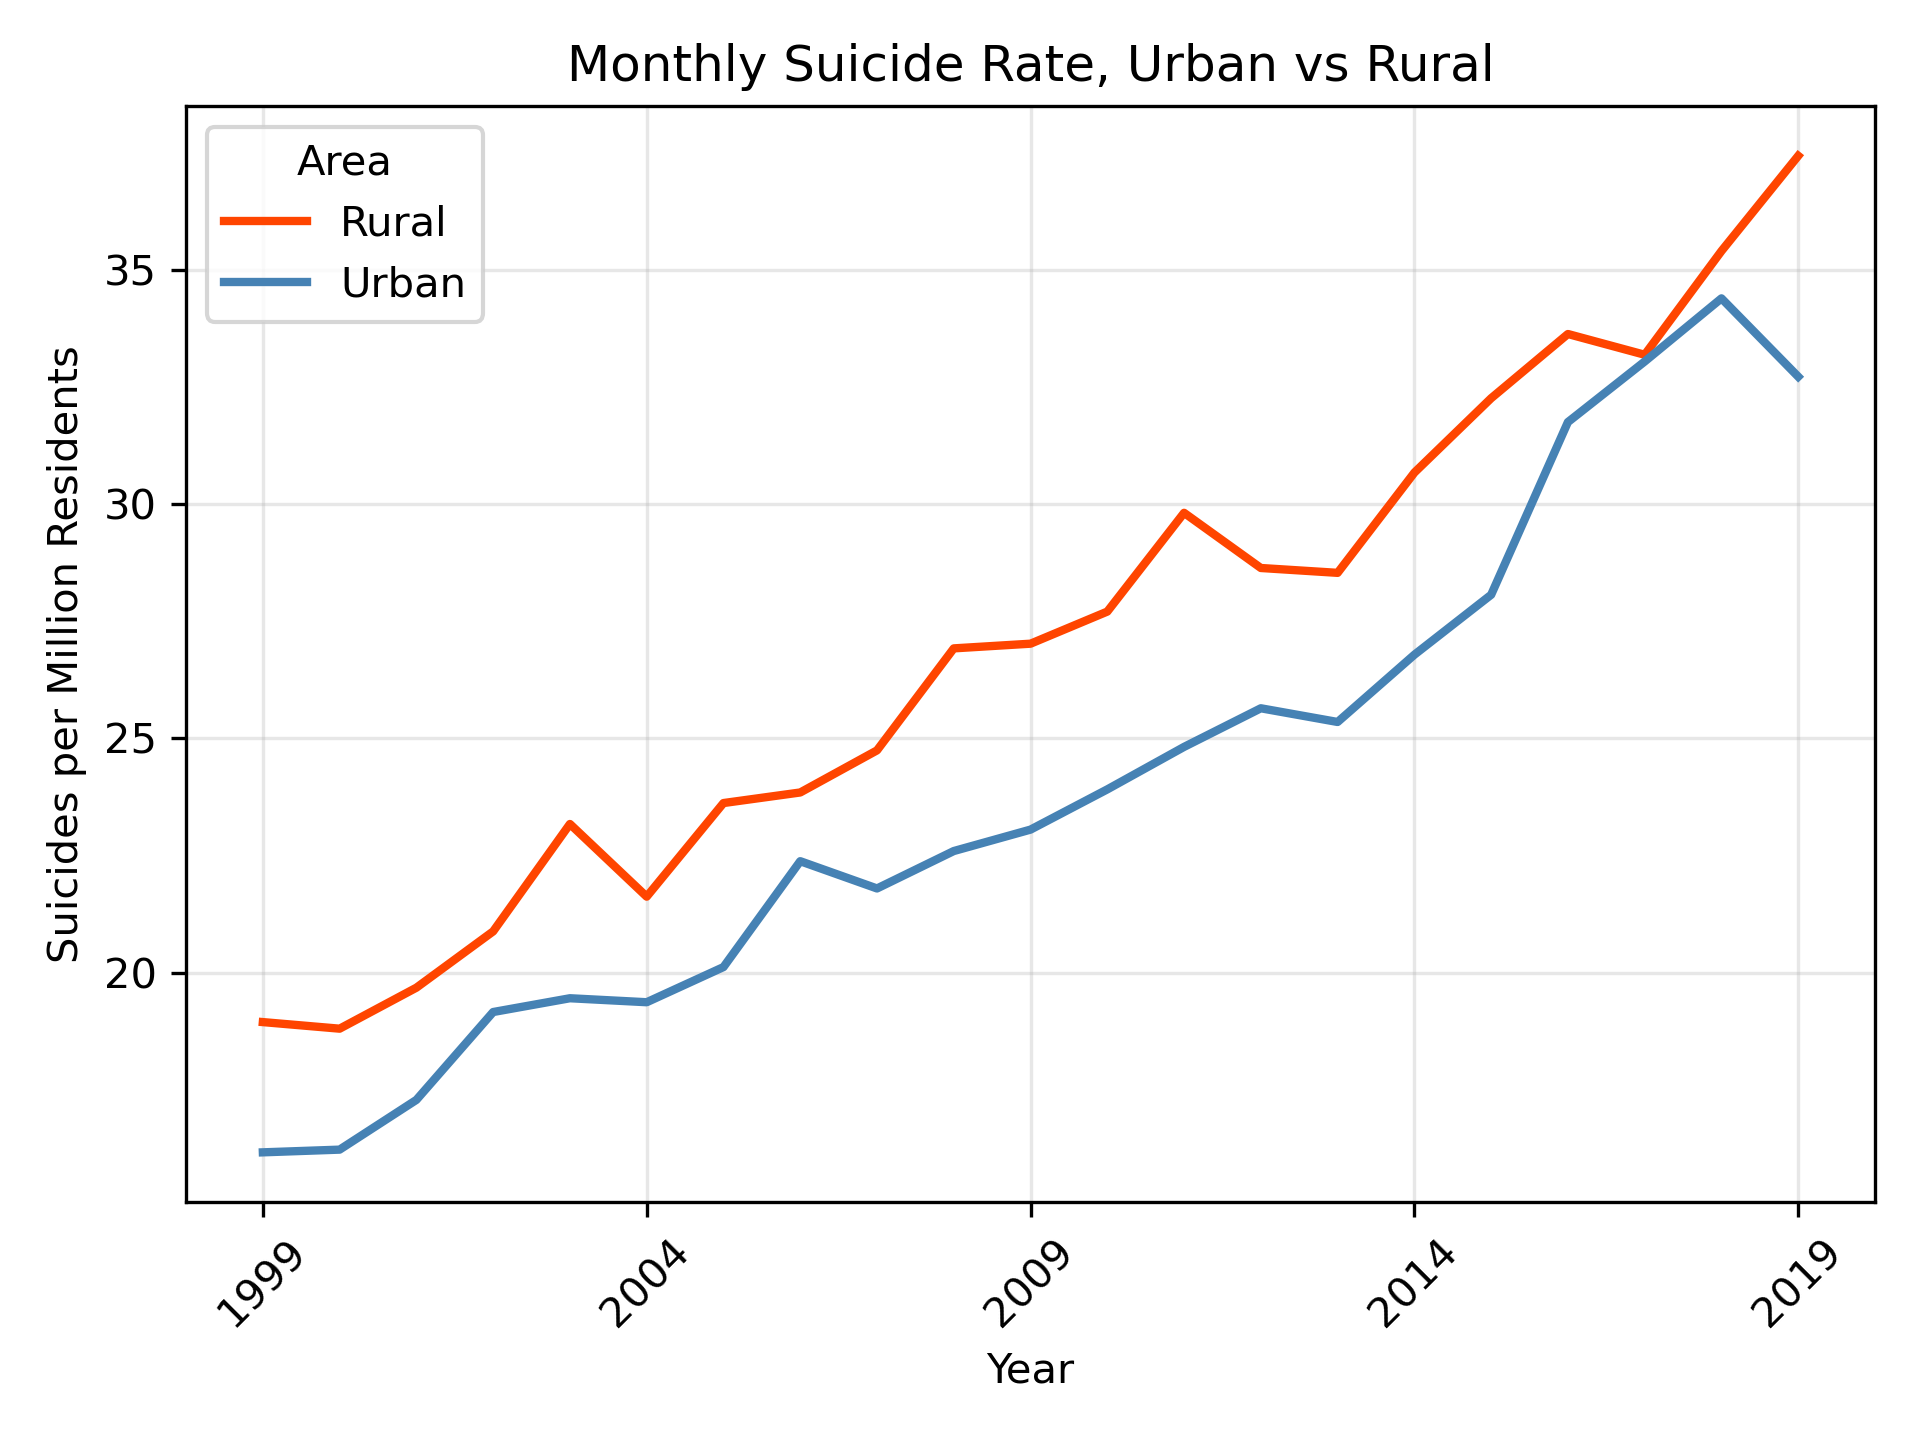
\includegraphics[width=\textwidth]{Monthly Suicide Rate.png}
        \caption{Monthly suicide rate, urban vs. rural}
        \label{fig:suicide}
    \end{subfigure}
    \hfill
    % Second subfigure
    \begin{subfigure}[b]{0.48\textwidth}
        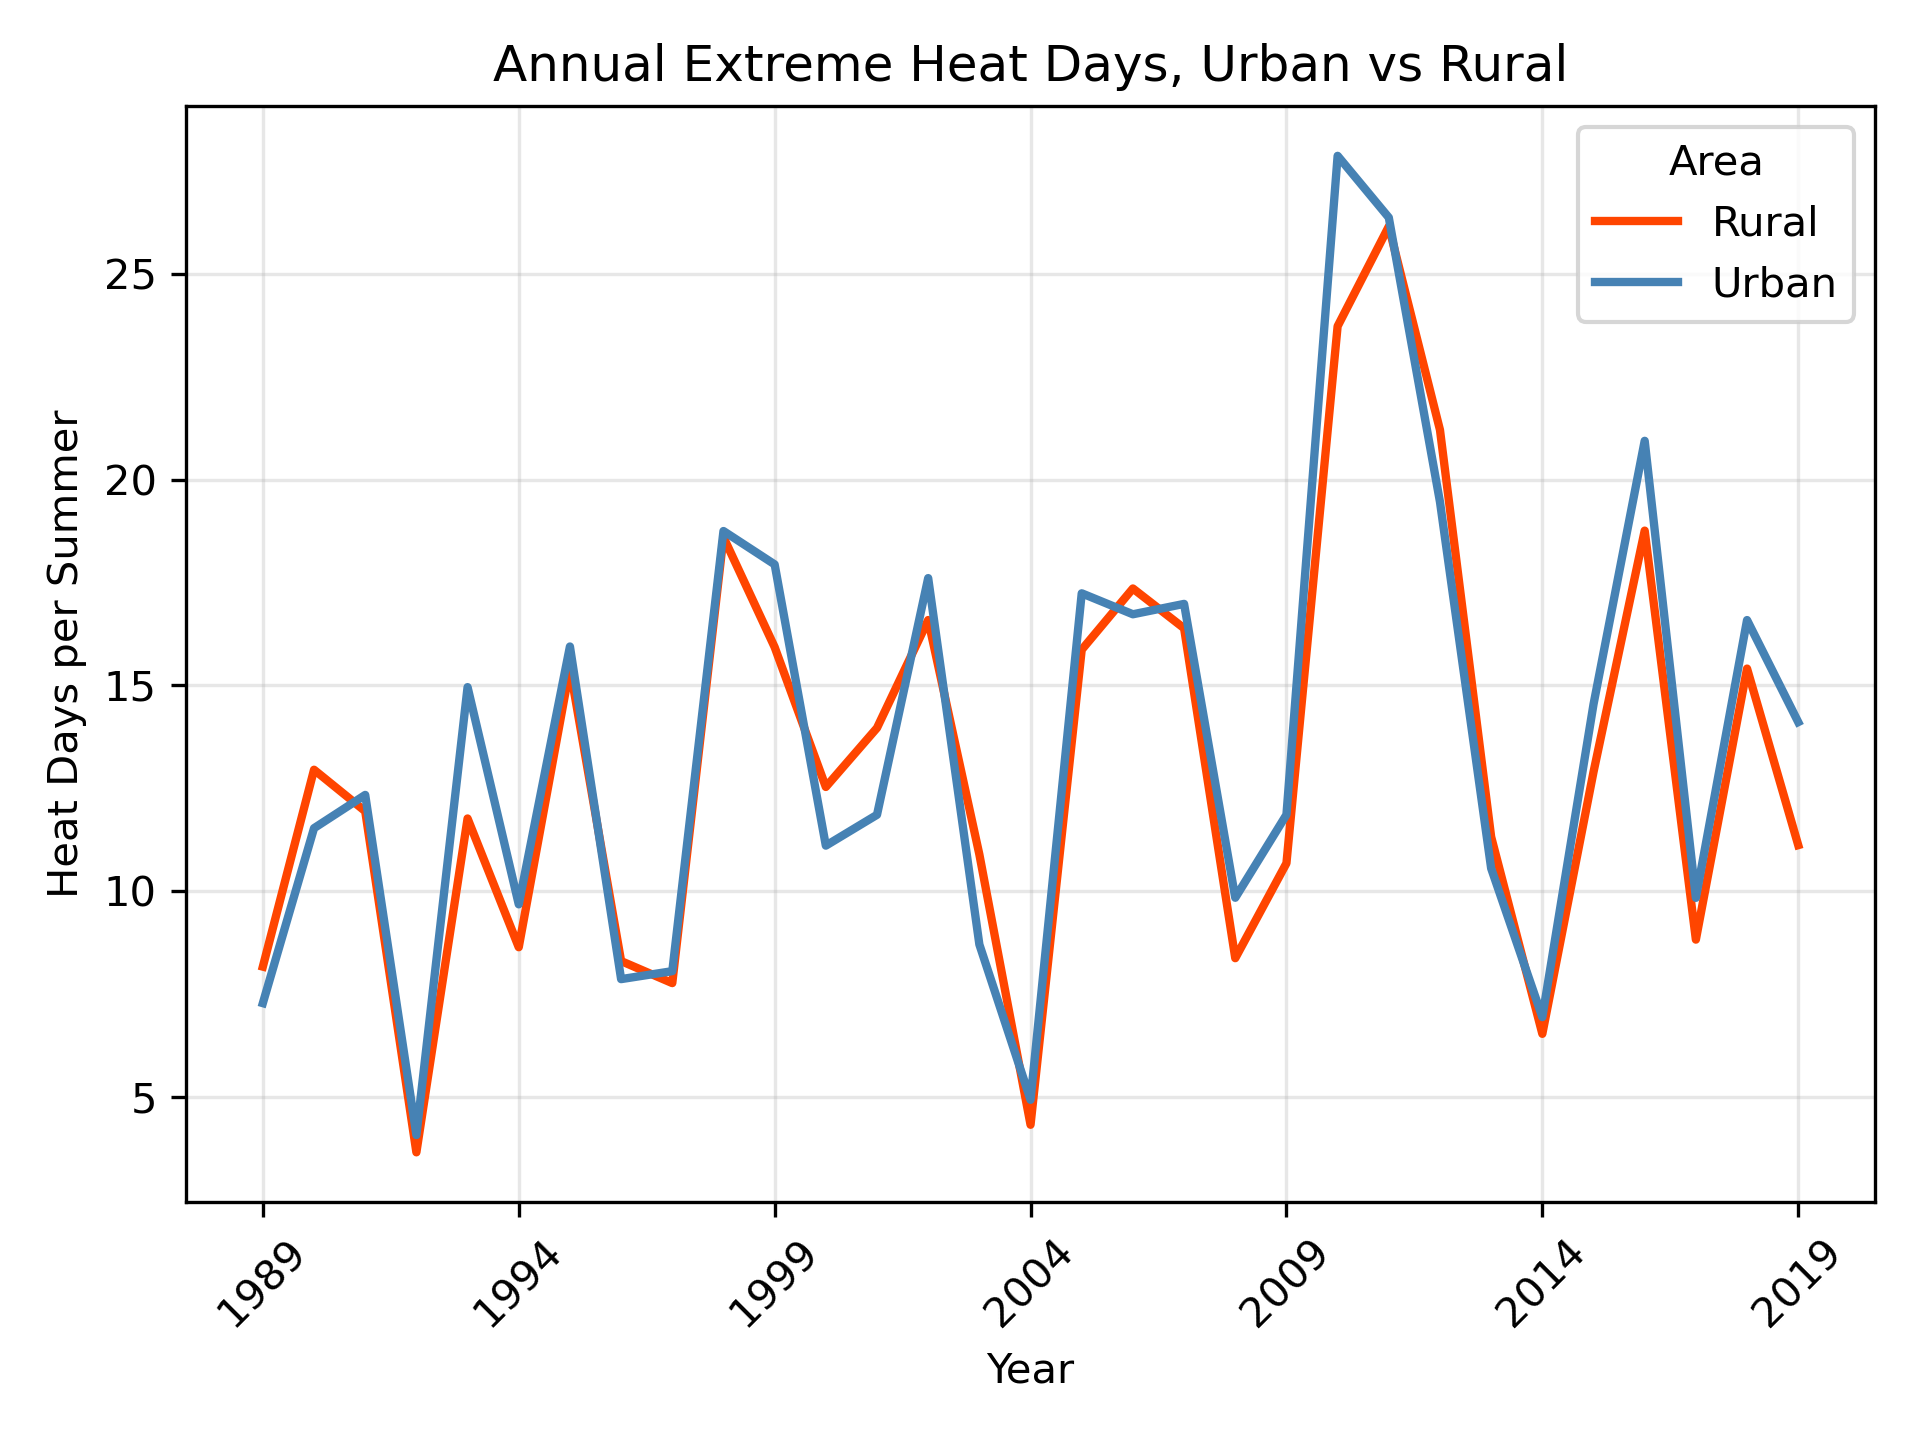
\includegraphics[width=\textwidth]{EHDs.png}
        \caption{Annual extreme heat days, urban vs. rural}
        \label{fig:ehds}
    \end{subfigure}
    
    \caption{Trends in suicide rates and extreme heat days across urban and rural areas.}
    \label{fig:trends}
\end{figure}

Fourth, the use of a granular, county-level panel dataset allows me to exploit both spatial and temporal variation in extreme heat exposure. By applying fixed effects and controlling for time trends at multiple levels, I am able to isolate the short-term causal effect of an extreme heat day on mental health mortality, while also exploring heterogeneity across urban and rural settings and demographic subgroups.

\section{Data and Methodology}
\subsection{Population Data}
County-level population data was used to calculate death rates and for regression weighting purposes. Subgroup county population data by sex, age, and race are obtained from the Surveillance, Epidemiology, and End Results Program \cite{seerPop2022}. I supplement this with county-level educational attainment data from the Economic Research Service branch of the US department of Agriculture that reports the number of adults 25+ in each educational attainment group (high school or less, some college or more) for 1980, 1990, 2000, and a 5 year average for 2016-2020 \cite{ersEducation2022}. For each county, I linearly interpolate from 1980 to 2020 to construct annual estimates of county-level education attainment for 1989-2019. I then calculate the death rate as standard.

\subsection{Mortality Data}
Data on monthly health related deaths at the county level are derived from the restricted use Detailed Mortality-All County data; part of the Vital Statistics Data maintained by the NCHS and can become available via request and application from the Centers for Disease Control \cite{nchsRestrictedData2021}. The raw data acquired includes every death reported in the United States between 1989 and 2019, along with the primary cause of each. Cause of death was used to categorize deaths as mental health related if they were caused by suicide, injuries of undetermined intent, or accidental poisoning, firearm, train, or drowning, explicitly detailed in table \ref{tab:mentalhealth_icd} \cite{MHClassification}. For a given county in a given summer month each year, I counted the number of mental health related deaths, both overall and by subgroup. The set of subgroups includes sex (M,F), age (0-24, 25-64, 65+), race/origin (White and non-Hispanic, non-White or Hispanic), and educational attainment (high school diploma or less, some college credit or more). Analysis for educational attainment was limited to 25+ adults, as younger people may not have had time to get a college education. Group specific deaths rates are calculated in terms of number of deaths per million using group - specific population counts. All figures suppressed counties that observed fewer than 10 total or subgroup mental health related deaths for the study period but are still included in the analysis.

\subsection{Temperature Data}
Temperature data was obtained from the PRISM Climate Group \cite{prismClimate2022}, which reports high resolution gridded climate data. The PRISM data contains 4km by 4km gridded estimates of daily average temperature for the United States for from 1989-2019. I aggregated the daily average temperature data to the county level and then mapped the set of daily average county temperatures in a given month and year to the number of extreme heat days (described below in 2.5).

\subsection{Urbanization Classification}
Counties are classified as urban or rural according to the 2013 NCHS Urban-Rural Classification Scheme \cite{nchsUrbanRural2013}. This system assigns each county to one of six categories based on its level of urbanization. For my analysis, I define urban counties as those falling into the top three categories: large central metro, large fringe metro, and medium metro. Counties in the bottom three categories - small metro, micropolitan, and noncore - are considered rural.

\subsection{Empirical Approach}
I use a panel fixed effects regression to estimate the effect of smoke exposure on suicide rates:
\[
Y_{cym} =  \beta\cdot\text{EHD}_{cym} + \delta_{cm} +\delta_{cy} +\delta_{ym} +\epsilon_{cym},
\]
\[
\text{where EHD}_{cym}=\sum_{d=1}^{|m|_y}\mathds{1}(T_{cymd}>P_{85,cm} \lor T_{cymd}>30\degree\text{C})
\]
$Y_{cym}$ is the defined suicide rate with deaths by suicide per million in county $c$, year $y$, and month $m$. $\text{EHD}_{cym}$ denotes the number of days in the same county-year-month where the average daily temperature exceeded either the 85th percentile threshold for that county-month or 30$\degree$C. Percentile thresholds are calculated separately for each county and month, using historical daily temperature data from 1989 to 2019. $\delta_{cm}$ represents county-by-month fixed effects, which subtract the county-specific monthly average from both suicide rates and EHDs. This ensures that identification comes from within-county deviations, comparing county-months in relatively low-EHD years to the same county-months in relatively high-EHD years. My main specification also includes county-year fixed effects, $\delta_{cy}$, which control for all county-specific factors that vary annually but not within a year (e.g., changes in economic conditions, demographic shifts). This prevents the need to separately control for county-level time-varying covariates. I also include year-month fixed effects, $\delta_{ym}$ which account for shocks common to all counties in a given month and year (such as the impacts of the 2008 financial crisis or coding changes like the ICD-10 transition). All regressions are weighted by 2000 Census county populations to account for differences in county size, and standard errors are clustered at the county level to allow for arbitrary serial correlation in the error terms within counties.


\section{Results}
I begin by presenting the estimated relationship between EHDs and suicide rates based on the baseline fixed effects regression model described in section 2.5.

\begin{figure}[ht]
    \centering
    \caption{Effect of one additional EHD on monthly suicide rates, by subgroup.}
    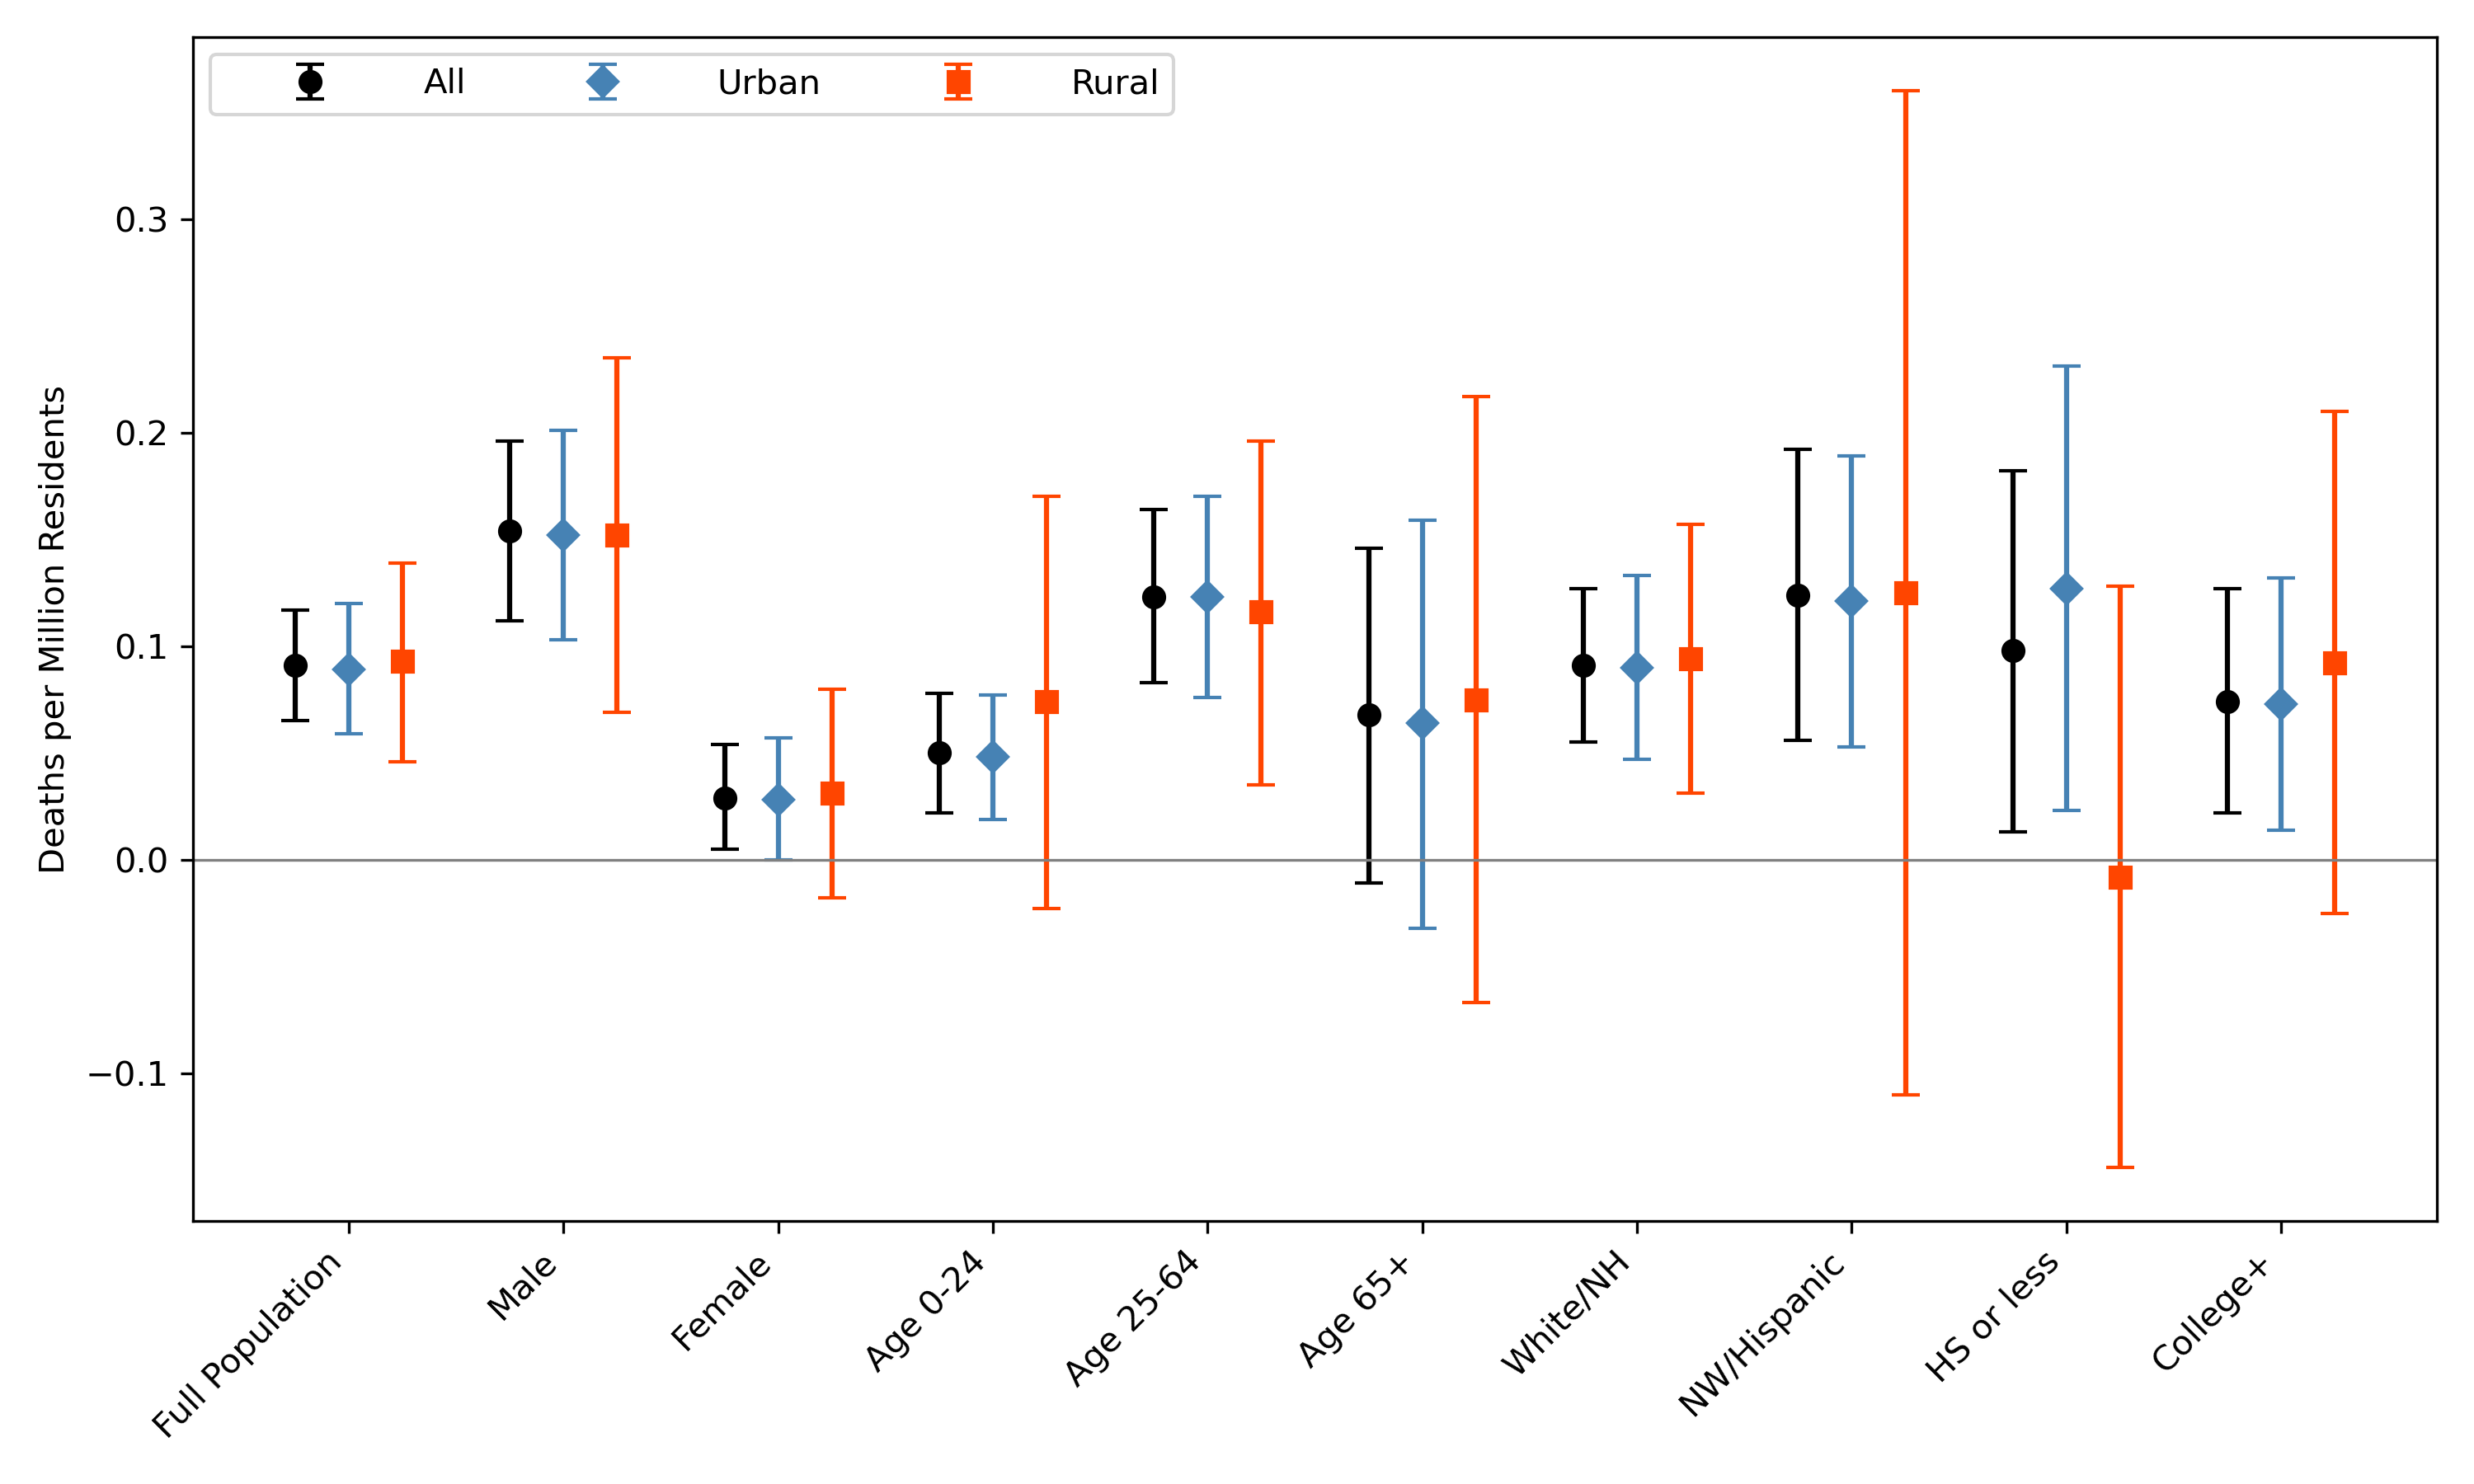
\includegraphics[width=\textwidth]{lin_results.png}
    \label{fig:lin_results}
\end{figure}
The markers indicate point estimates while the lines the 95\% CI estimates of the indicated relationships. Estimates for each population subgroup and area type are taken from separate regressions based on population subgroup-specific suicide rates in the indicated sample of counties. “White/NH” refers to those who are White and non-Hispanic, and “NW/Hispanic” is the converse (non-White or Hispanic). “HS or less” refers to adults 25 years and older with a high school diploma or less, and “College+” refers to adults 25 years and older with some college credits or more. 

For robustness, results were validated using Poisson regression models, where coefficients capture proportional changes rather than absolute changes in suicide rates. The Poisson models produced similar directional findings across subgroups, although the magnitudes of the effects differed somewhat between urban and rural counties. These differences likely reflect the influence of lower baseline suicide rates in certain areas, which can affect proportional versus absolute change estimates. Overall, the consistency in the direction of effects across specifications reinforces the robustness of the main findings. Results are more unstable among rural areas due to count sizes. Regression estimates and mean suicide rates for each subgroup are reported in the Appendix, tables \ref{tab:lin_reg_summary} and \ref{tab:poisson_reg_summary}.


\section{Discussion}

My results demonstrate that exposure to EHDs increases suicide mortality in the United States. I estimate that one additional EHD in a summer month leads to an increase of 0.091 suicide deaths per million residents. This corresponds to a 0.37\% rise relative to the baseline monthly suicide rate of 25.68 per million. While modest in absolute terms, this effect may accumulate meaningfully as extreme heat events become more frequent and intense under climate change, and with our definition of an EHD, this may serve as a possible lower bound. The economic implications are also significant, given the high direct and indirect costs associated with suicide and mental health-related deaths.

The effect is slightly more pronounced in rural populations and among demographic groups with elevated baseline suicide risk, including men and working-age adults. These findings suggest that extreme heat may exacerbate existing vulnerabilities, potentially widening existing mental health disparities.

Several mechanisms could explain the observed relationship. Physiological stress from heat can aggravate mental health disorders, disrupt sleep, and increase irritability and impulsivity \cite{Hsiang2013}. These pathways may be particularly salient for individuals in lower socioeconomic groups, who are more likely to engage in outdoor labor or lack access to cooling resources. 

The observed association between extreme heat and suicide highlights the often-overlooked mental health dimension of climate change. If current trends in temperature extremes continue, the mental health burden could grow considerably. These findings underscore the need for targeted public health interventions-such as early warning systems, mental health outreach, and access to cooling infrastructure—especially in high-risk communities. Interestingly, although rural communities face higher baseline suicide risk, urban areas tend to experience more severe heat exposure. This contrast may help explain the similarity in urban and rural point estimates, as greater heat intensity in urban areas could offset lower baseline vulnerability.

\subsection{Limitations}

Several limitations of this study should be acknowledged. First, for the definition of EHD, the analysis was limited to summer months (June, July, and August). While this approach captures periods with the highest likelihood of extreme heat, it excludes potential effects of unseasonal heat spikes in spring or fall, potentially underestimating the overall impact of temperature on mental health, particularly as suicides typically peak in spring \cite{bridges2005}.

Additionally, due to time constraints and data processing limitations, I did not account for shifting county boundaries or weighing temperatures by population centers within counties. These refinements could improve precision, particularly in counties with large or unevenly distributed populations. Also, the fixed-effects design controls for unobserved, time-invariant county characteristics, but I did not incorporate models without fixed effects for comparison. Additionally, the analysis does not consider potential lagged effects of extreme heat on suicide risk, which could occur over multiple weeks or months.

A further limitation concerns the definition of EHDs. The use of an 85th percentile threshold captures heat anomalies relative to local historical norms rather than absolute levels of heat exposure. As a result,  even in the presence of broader climate warming, the number of extreme heat days defined this way may not show a consistent upward trend over time, as percentile thresholds themselves shift upward. Consequently, this measure may primarily reflect interannual variability rather than long-term warming trends. While this approach is valuable for identifying short-term deviations most likely to impact human health, it may underestimate the cumulative burden of rising temperatures over the study period. The true effects are likely more severe.

\section{Future Directions}
Future research should expand upon this work by examining the effects of temperature extremes across all months of the year, potentially uncovering significant impacts during transitional seasons such as spring and fall. Additional studies incorporating dynamic models and lagged temperature effects would provide deeper insights into the temporal dynamics of heat-related mental health outcomes. Furthermore, refining temperature measures by weighting for population centers and accounting for shifting county boundaries could enhance precision and robustness. Lastly, exploring alternative temperature thresholds or extreme definitions and their varying health impacts would further elucidate how incremental climatic shifts influence mental health outcomes.

\section{Replication}
This analysis relies on the Restricted-Use Vital Statistics Data from the Centers for Disease Control and Prevention. Access to this data can be obtained by following the instructions at which can be found here: \cite{nchsRestrictedData2021}. Other public data and my code can be found here (still working on this).
\newpage
\section{Appendix}
\appendix
\renewcommand{\thefigure}{A.\arabic{figure}}
\setcounter{figure}{0}

\begin{figure}[H]
    \centering
    \caption{Average Monthly Suicide Rate(Deaths per Million) by County}
    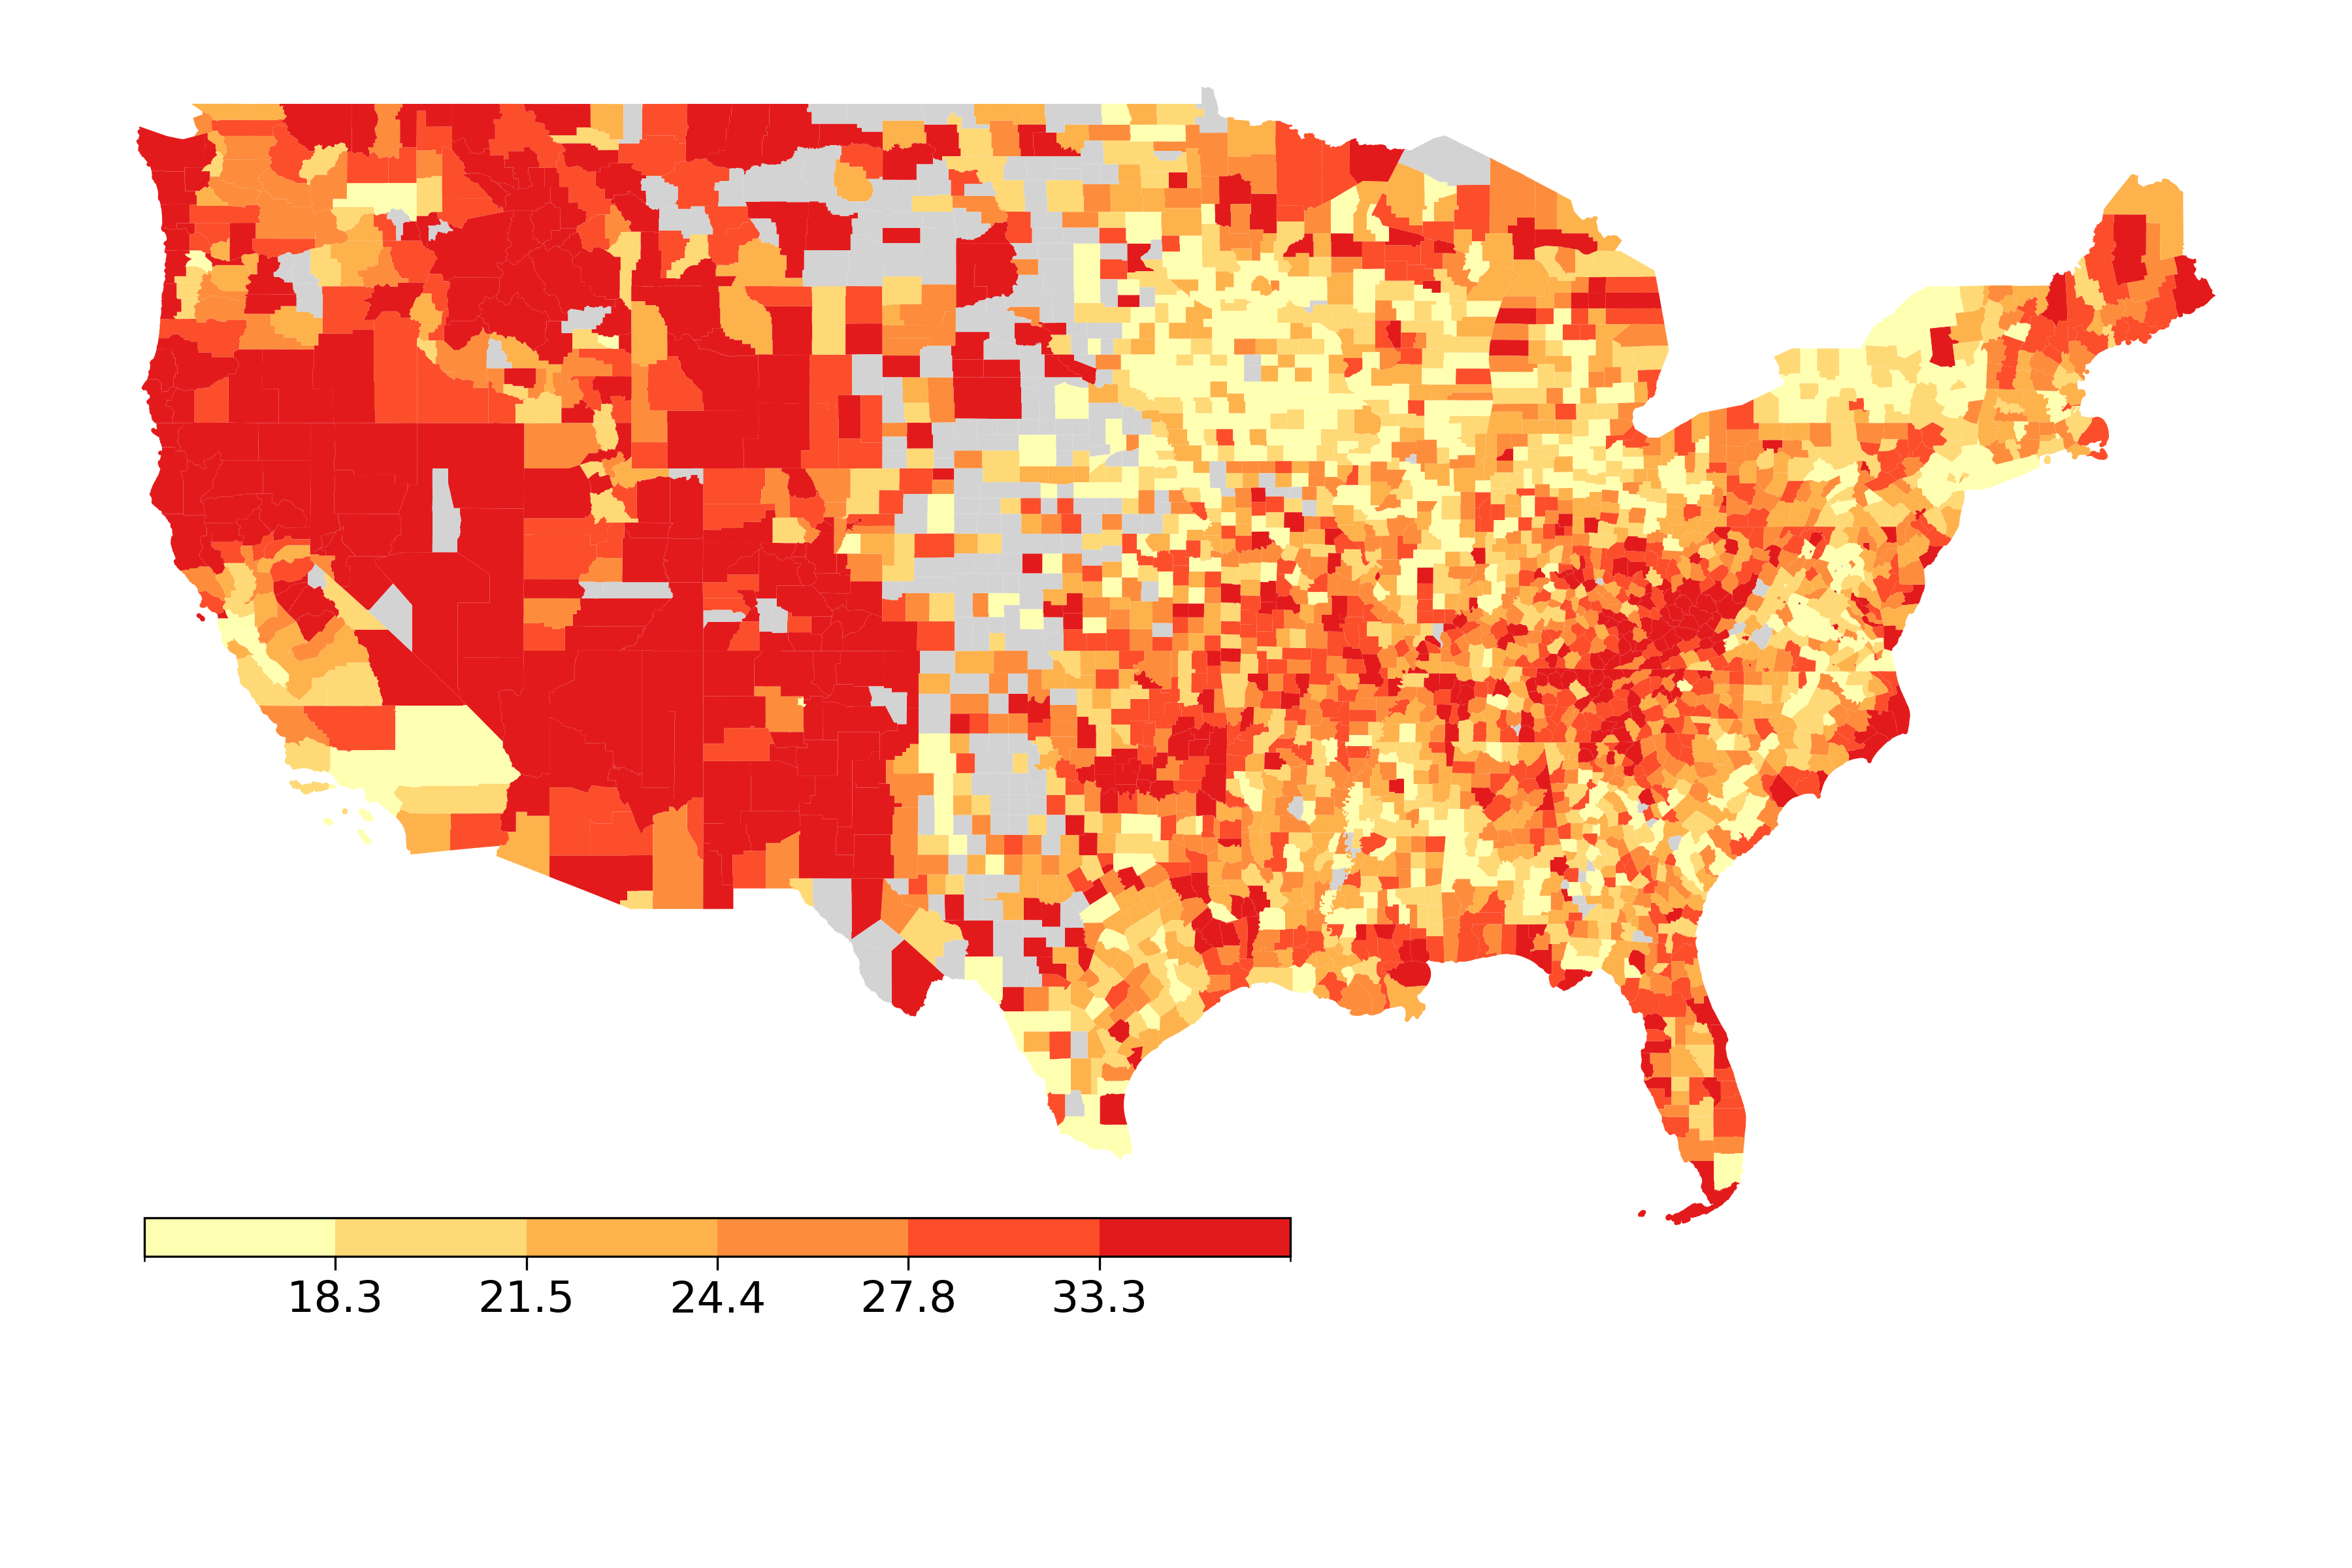
\includegraphics[width=0.9\textwidth]{suicide map.png}
    \label{fig:suicide_map}
\end{figure}


\begin{figure}[H]
    \centering
    \caption{Average Summer Percentile Thresholds(°C) by County}
    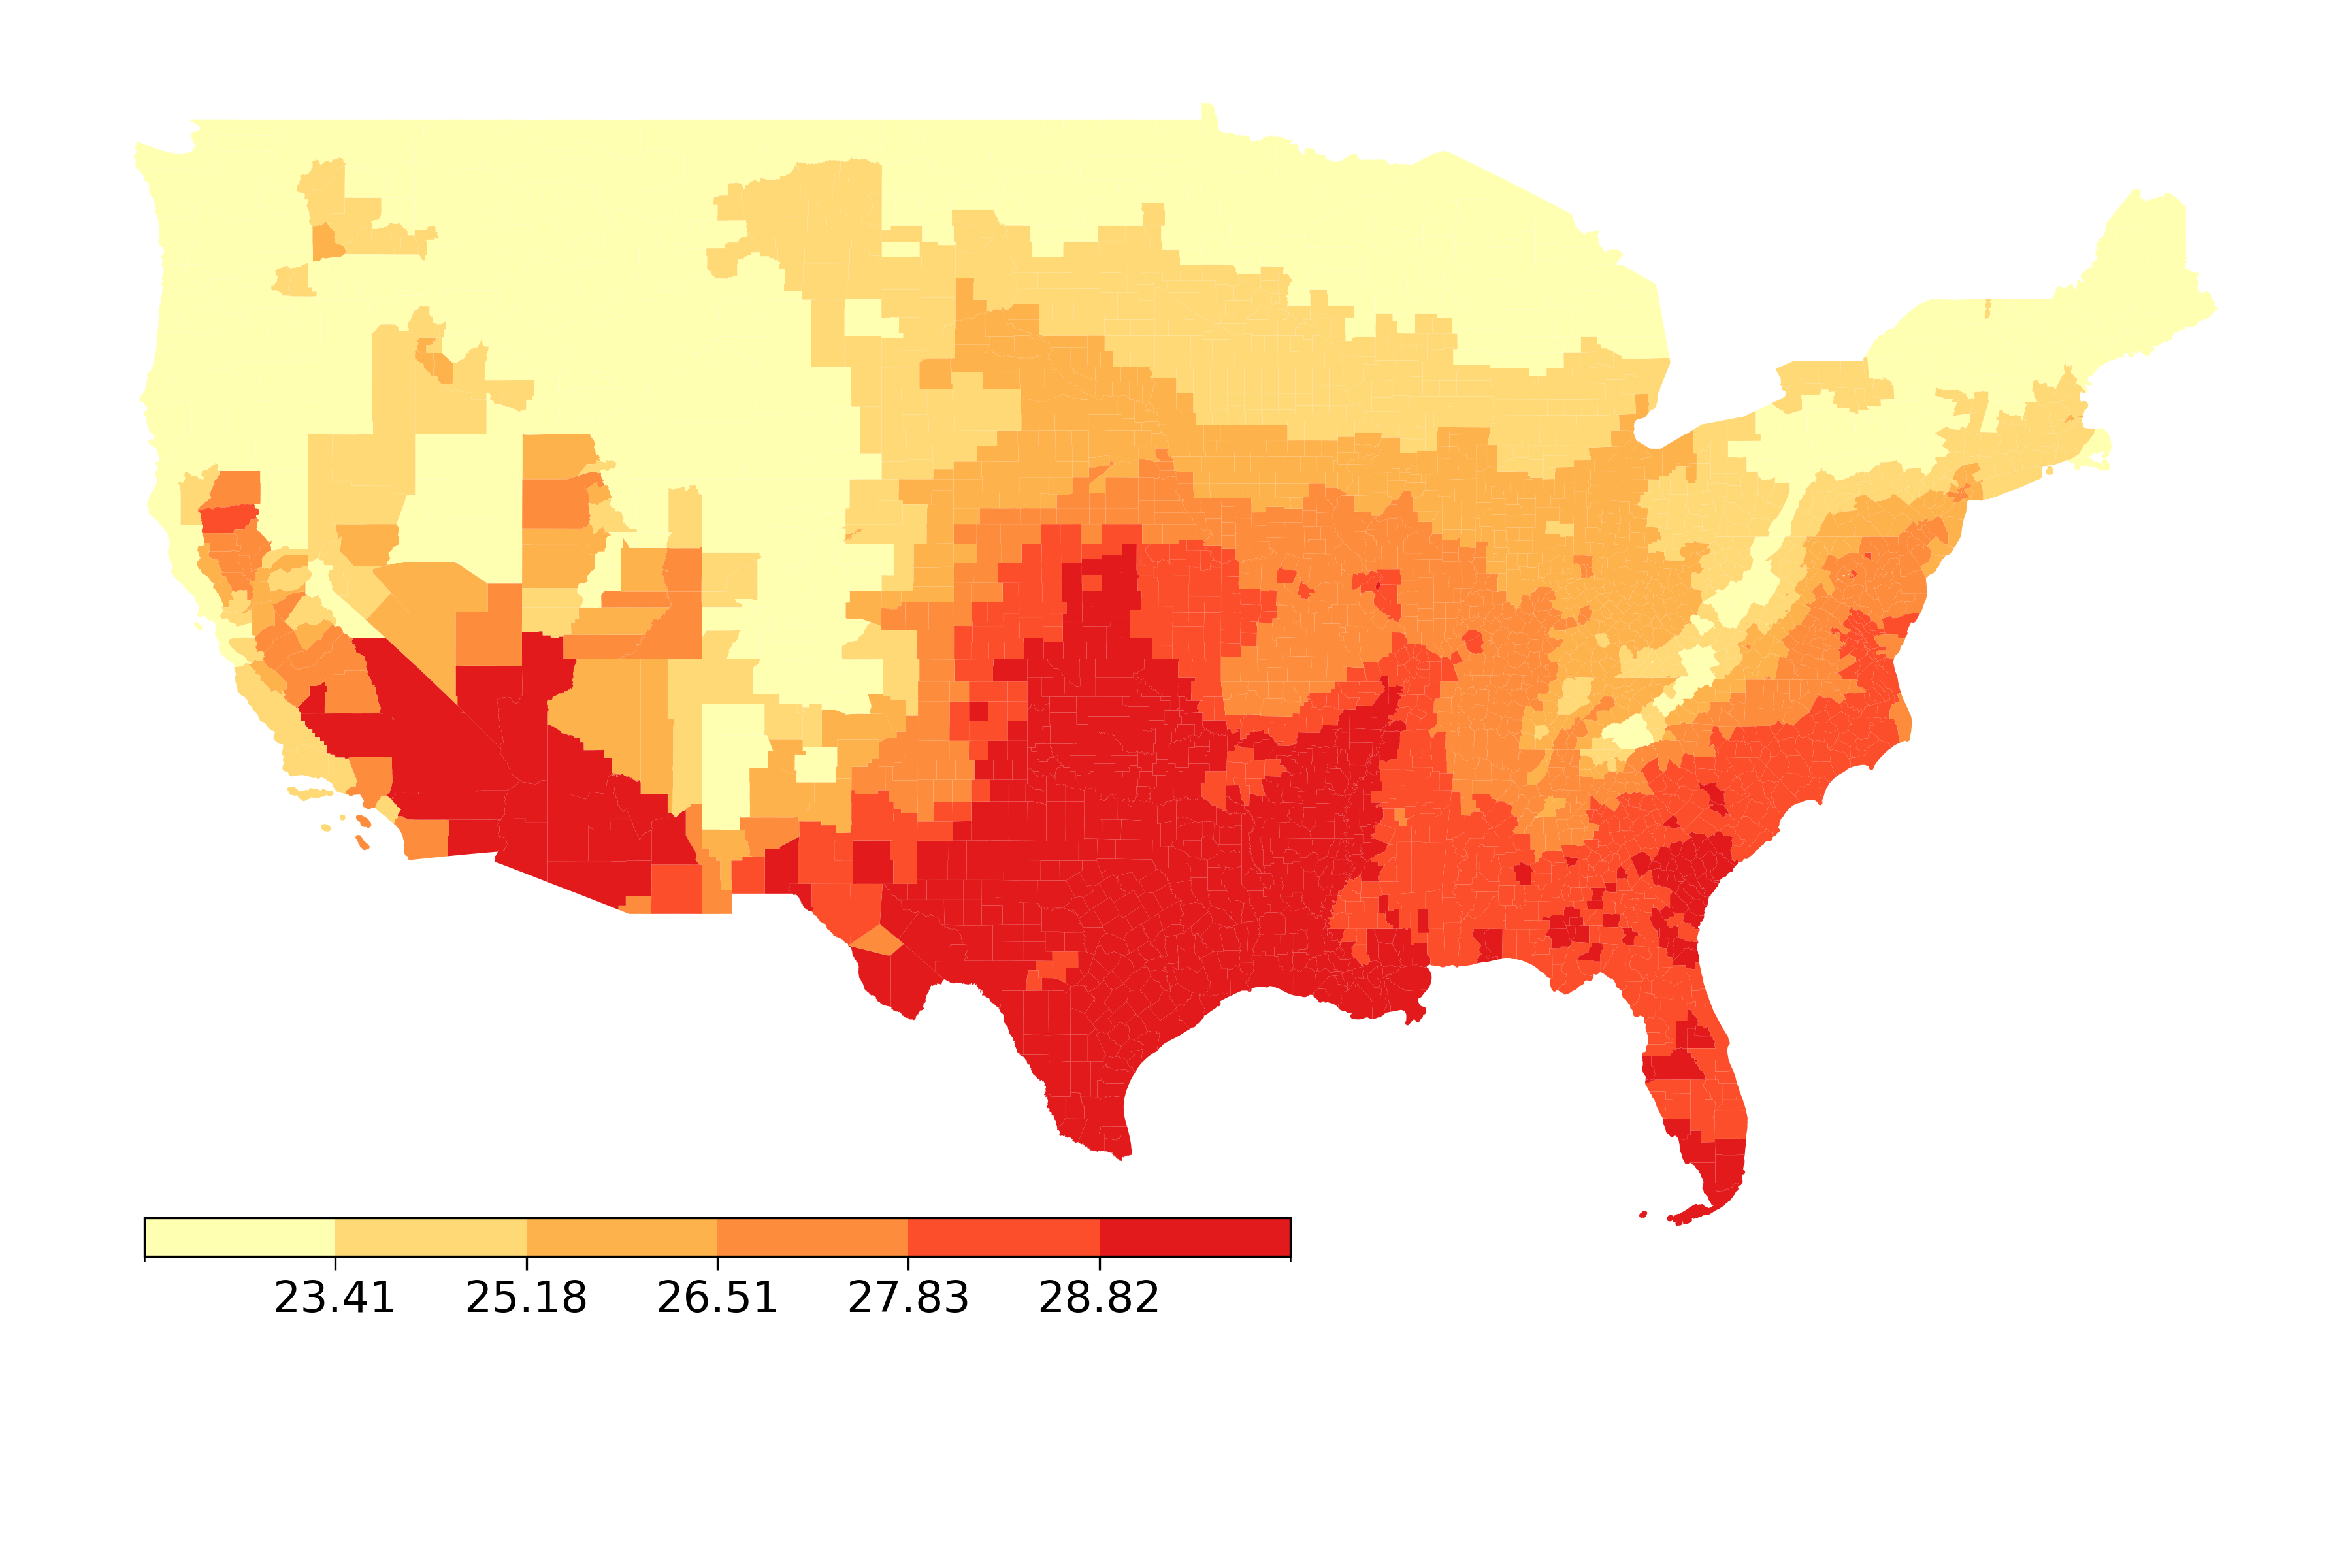
\includegraphics[width=0.9\textwidth]{thresholds.png}
    \label{fig:thresholds_map}
\end{figure}

%\section{Trends in Suicide and EHDs}
\begin{figure}[H]
    \centering
    \begin{subfigure}[b]{0.48\textwidth}
        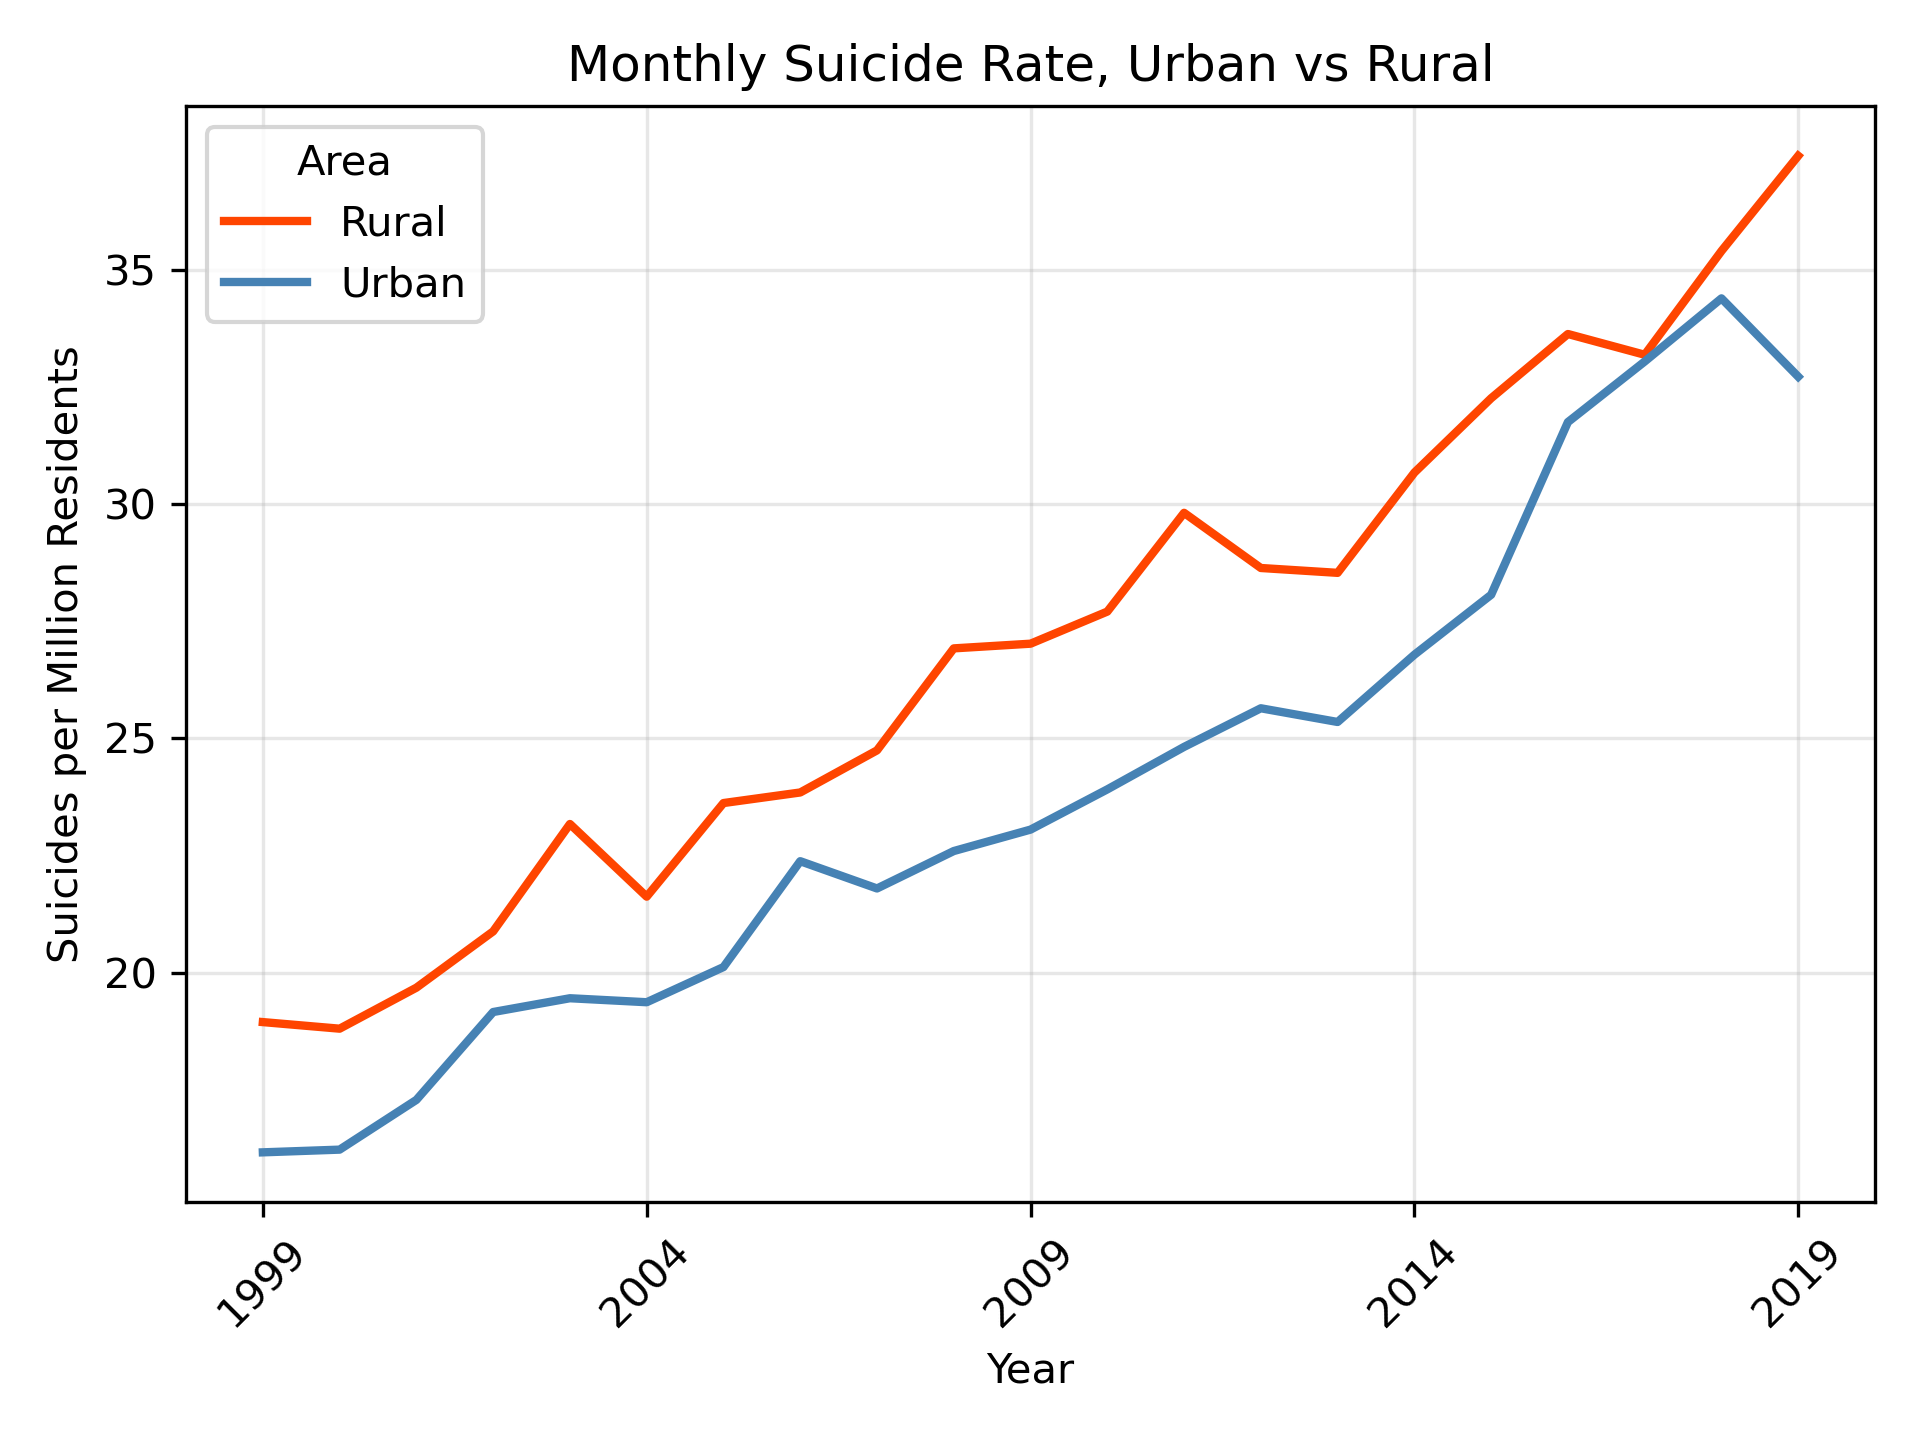
\includegraphics[width=\textwidth]{Monthly Suicide Rate.png}
        \caption{Monthly suicide rate, urban vs. rural}
        \label{fig:suicide}
    \end{subfigure}
    \hfill
    % Second subfigure
    \begin{subfigure}[b]{0.48\textwidth}
        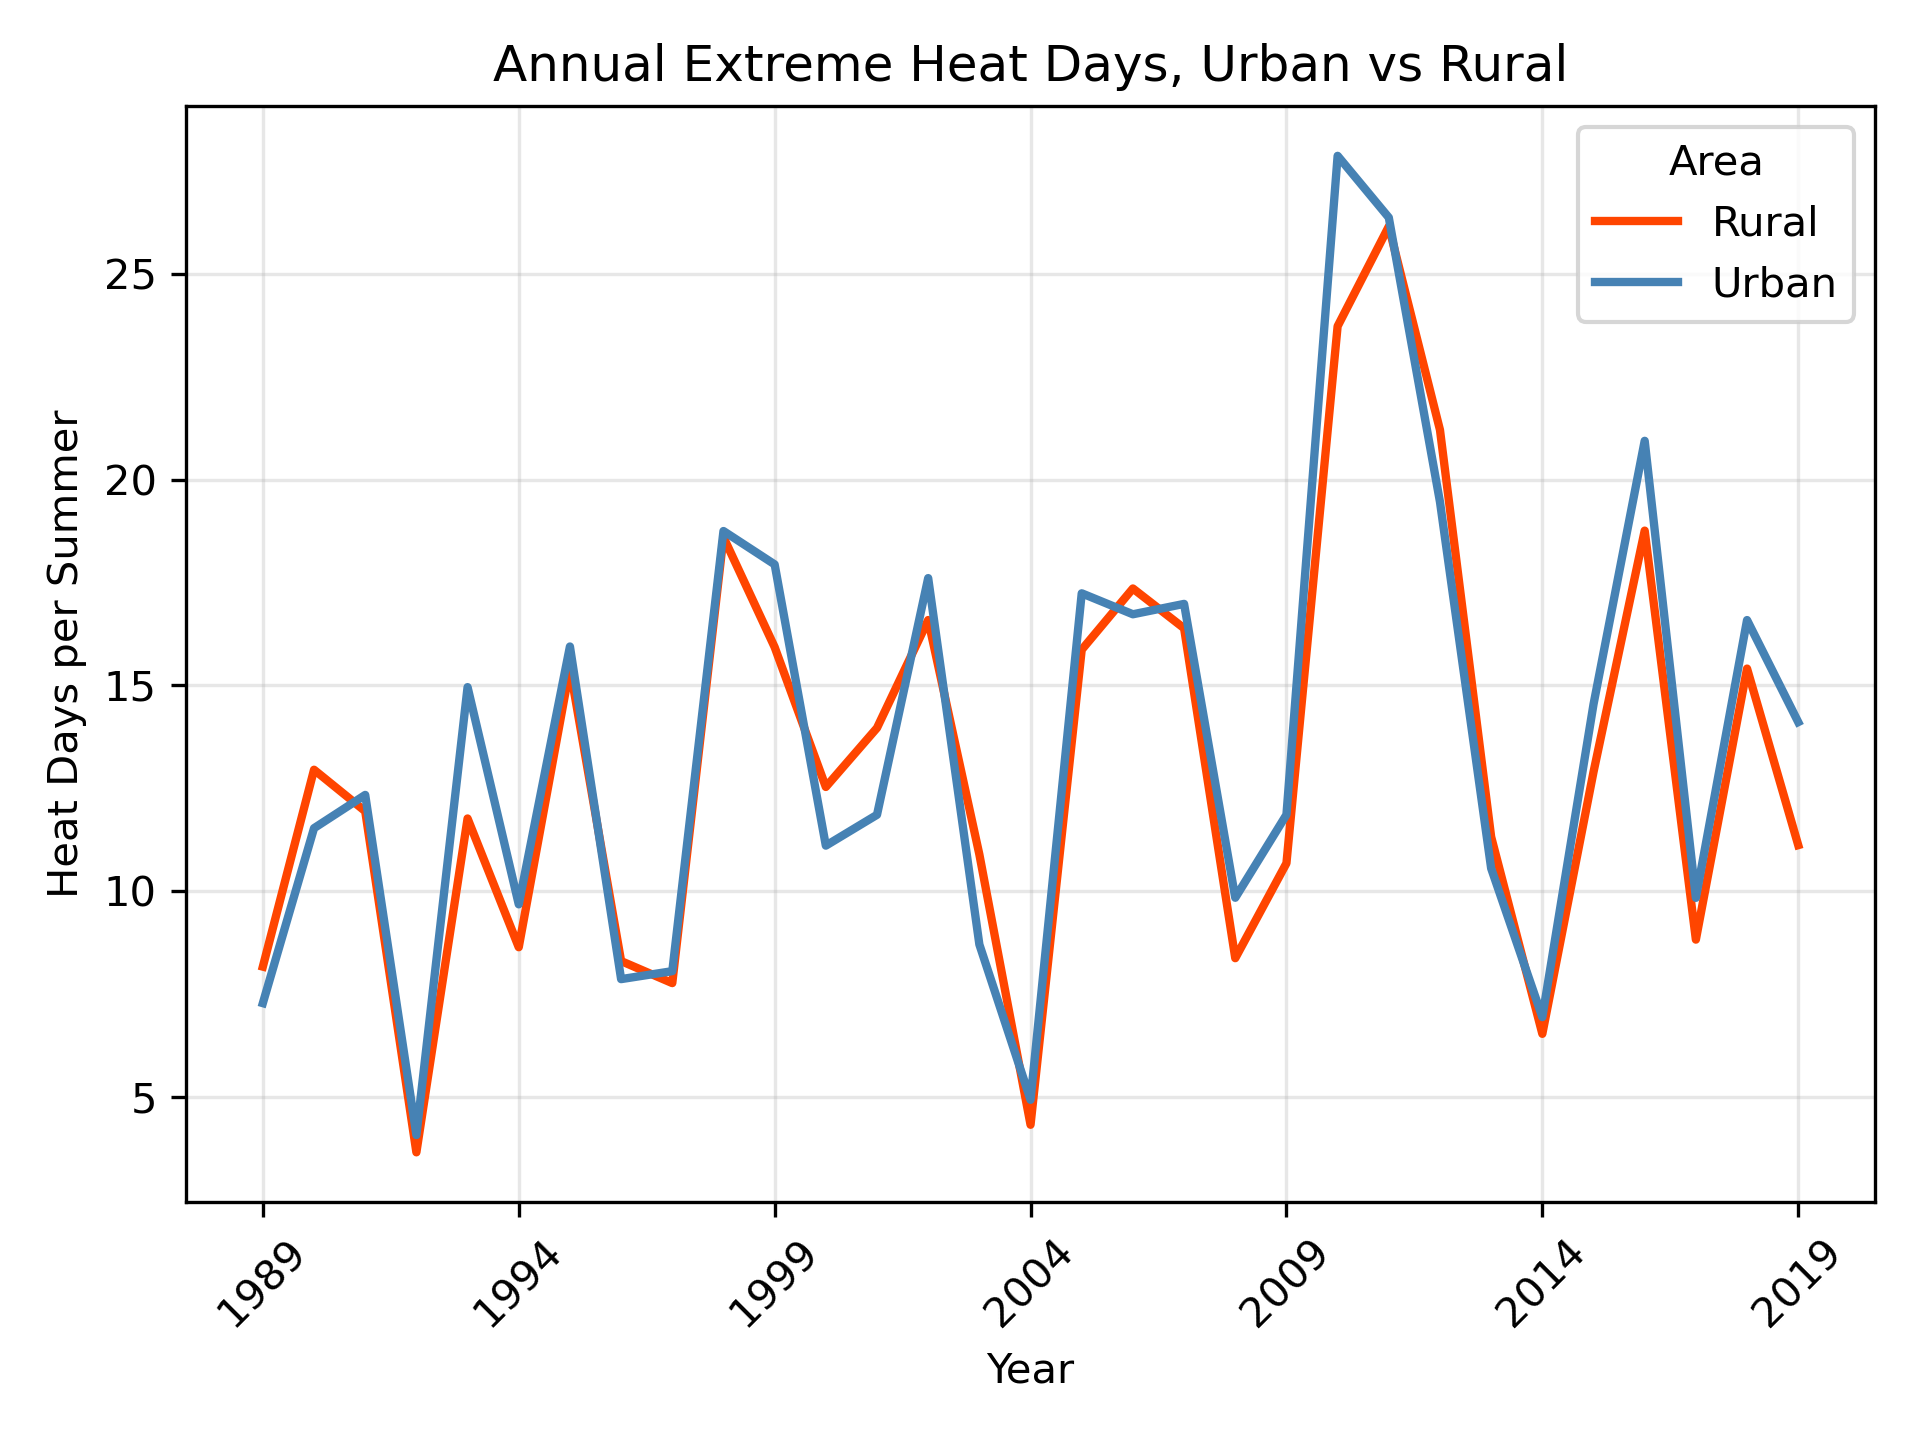
\includegraphics[width=\textwidth]{EHDs.png}
        \caption{Annual extreme heat days, urban vs. rural}
        \label{fig:ehds}
    \end{subfigure}
    
    \caption{Trends in suicide rates and extreme heat days across urban and rural areas.}
    \label{fig:trends}
\end{figure}

\begin{figure}[ht]
    \centering
    \caption{Effect of one additional EHD on monthly suicide rates, by subgroup.}
    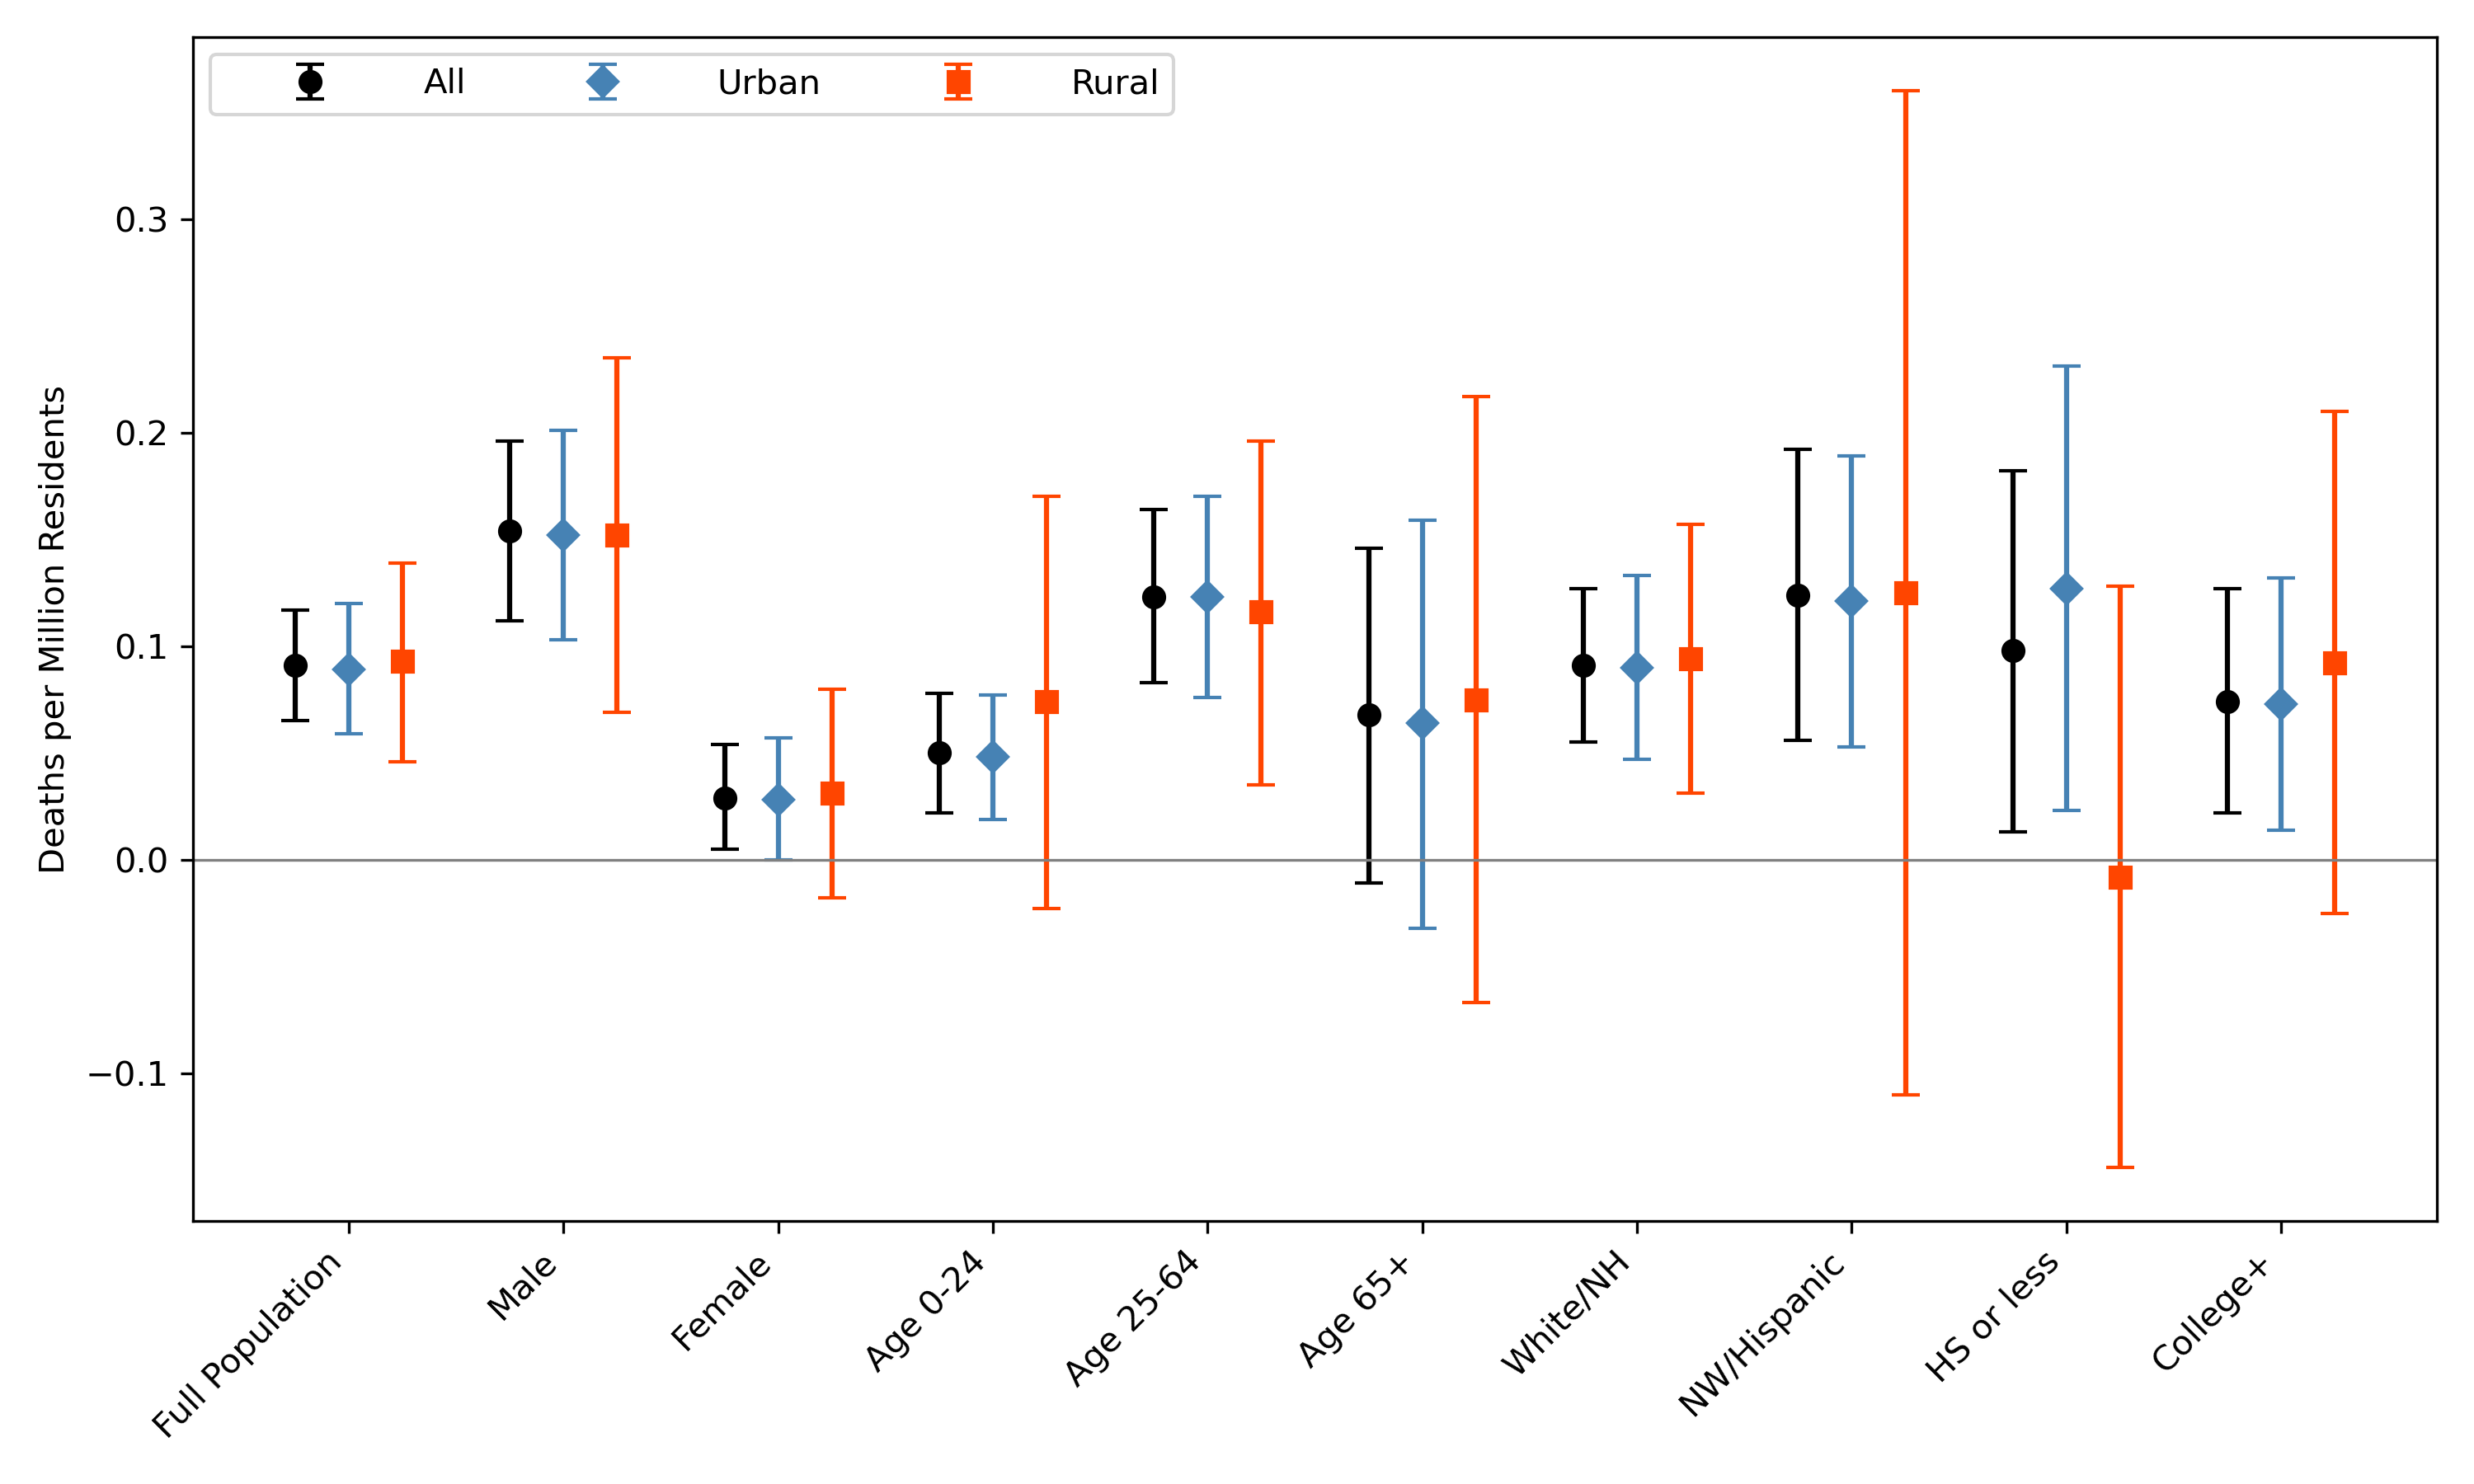
\includegraphics[width=\textwidth]{lin_results.png}
    \label{fig:lin_results}
\end{figure}

%\section{ICD Codes for Mental Health-Related Mortality}
\begin{table}[H]
\centering
\caption{ICD-9 and ICD-10 Codes Included in Mental Health–Related Mortality} % <-- YOU NEED caption!
\label{tab:mentalhealth_icd} % label always after caption
\begin{tabular}{|>{\raggedright\arraybackslash}p{3cm}|>{\raggedright\arraybackslash}p{5cm}|>{\raggedright\arraybackslash}p{5cm}|}
\hline
\textbf{Cause of Death} & \textbf{ICD-9 Codes} & \textbf{ICD-10 Codes} \\ \hline
Suicides & E950–E959 & Intentional self-harm: U03, X60–X84, Y87.0 \\ \hline
Injuries of Undetermined Intent & Injury undetermined whether accidentally or purposely inflicted: E980–E989 & Events of undetermined intent: Y10–Y34, Y87.2, Y89.9 \\ \hline
Accidental Poisonings & Accidental poisoning: E850–E869 & Accidental poisoning and exposure to noxious substances: X40–X49 \\ \hline
Accidental Drownings & Accidental drowning and submersion: E910 & Accidental drowning and submersion: W65–W74 \\ \hline
Accidental Firearms & Accident caused by handgun: E922.0 \newline Accident caused by other firearms: E922.1–E922.9 & Accidental discharge of firearms: W32–W34 \\ \hline
Train Accidents & Railway accidents: E800–E807 \newline Motor vehicle–train collisions: E810 & Railway accidents: V05, V15, V80.6, V81.2–V81.9 \newline Motor vehicle–train collisions: V25, V35, V45, V55, V65, V75, V81.0–V81.1, V87.6, V88.6 \\ \hline
\end{tabular}
\end{table}

\begin{table}[H]
\centering
\caption{Linear Estimates}
\label{tab:lin_reg_summary}
\begin{tabular}{llcc}
\toprule
\textbf{Region} & \textbf{Subgroup} & \textbf{Estimate (SE)} & \textbf{N} \\
\midrule
All & Full Population & $0.091^{***}$ (0.013) & 280639 \\
 & Male & $0.154^{***}$ (0.021) & 273493 \\
 & Female & $0.029^{**}$ (0.012) & 270697 \\
 & Age 0–24 & $0.05^{***}$ (0.014) & 118321 \\
 & Age 25–64 & $0.123^{***}$ (0.021) & 248305 \\
 & Age 65+ & $0.068^{*}$ (0.04) & 277220 \\
 & White/NH & $0.091^{***}$ (0.018) & 268352 \\
 & NW/Hispanic & $0.124^{***}$ (0.035) & 168295 \\
 & HS or less & $0.098^{**}$ (0.044) & 166512 \\
 & College+ & $0.064^{***}$ (0.027) & 142230 \\
Urban & Full Population & $0.089^{***}$ (0.016) & 73668 \\
 & Male & $0.152^{***}$ (0.025) & 73193 \\
 & Female & $0.028^{*}$ (0.015) & 72902 \\
 & Age 0–24 & $0.048^{***}$ (0.015) & 48897 \\
 & Age 25–64 & $0.123^{***}$ (0.024) & 71476 \\
 & Age 65+ & $0.064^{}$ (0.049) & 73324 \\
 & White/NH & $0.09^{***}$ (0.022) & 70964 \\
 & NW/Hispanic & $0.121^{***}$ (0.035) & 59547 \\
 & HS or less & $0.127^{**}$ (0.053) & 44942 \\
 & College+ & $0.073^{**}$ (0.03) & 42168 \\
Rural & Full Population & $0.093^{***}$ (0.024) & 206971 \\
 & Male & $0.152^{***}$ (0.042) & 200300 \\
 & Female & $0.031^{}$ (0.025) & 197795 \\
 & Age 0–24 & $0.074^{}$ (0.049) & 69424 \\
 & Age 25–64 & $0.116^{***}$ (0.041) & 176829 \\
 & Age 65+ & $0.075^{}$ (0.073) & 203896 \\
 & White/NH & $0.094^{***}$ (0.032) & 197388 \\
 & NW/Hispanic & $0.125^{}$ (0.12) & 108748 \\
 & HS or less & $-0.008^{}$ (0.069) & 121570 \\
 & College+ & $0.092^{}$ (0.06) & 100062 \\
\bottomrule
\end{tabular}
\vspace{0.5em}
\begin{flushleft}
\footnotesize
\textit{Notes}: This table shows linear regression estimates of the effect of extreme heat days on suicide rates per million. Standard errors are in parentheses. All models include county-month, county-year, and year-month fixed effects, and are weighted by 2000 county population. Standard errors are clustered at the county level.\\
$^{*}p<0.1$, $^{**}p<0.05$, $^{***}p<0.01$.
\end{flushleft}
\end{table}

\begin{table}[H]
\centering
\caption{Poisson Estimates}
\label{tab:poisson_reg_summary}
\begin{tabular}{llcc}
\toprule
\textbf{Region} & \textbf{Subgroup} & \textbf{IRR (SE)} & \textbf{N} \\
\midrule
All & Full Population & $1.004^{***}$ (0.001) & 211090 \\
 & Male & $1.004^{***}$ (0.001) & 193568 \\
 & Female & $1.002^{}$ (0.001) & 123330 \\
 & Age 0–24 & $1.005^{**}$ (0.002) & 73148 \\
 & Age 25–64 & $1.004^{***}$ (0.001) & 173273 \\
 & Age 65+ & $1.003^{}$ (0.002) & 105106 \\
 & White/NH & $1.003^{***}$ (0.001) & 193367 \\
 & NW/Hispanic & $1.005^{***}$ (0.002) & 75249 \\
 & HS or less & $1.003^{}$ (0.002) & 103545 \\
 & College+ & $1.005^{*}$ (0.003) & 57557 \\
 Urban & Full Population & $1.004^{***}$ (0.001) & 67301 \\
 & Male & $1.005^{***}$ (0.001) & 64643 \\
 & Female & $1.002^{}$ (0.002) & 51888 \\
 & Age 0–24 & $1.005^{**}$ (0.002) & 38406 \\
 & Age 25–64 & $1.004^{***}$ (0.001) & 62040 \\
 & Age 65+ & $1.003^{}$ (0.002) & 44665 \\
 & White/NH & $1.003^{***}$ (0.001) & 63530 \\
 & NW/Hispanic & $1.005^{***}$ (0.002) & 37765 \\
 & HS or less & $1.003^{}$ (0.002) & 36532 \\
 & College+ & $1.005^{*}$ (0.003) & 27118 \\
Rural & Full Population & $1.003^{**}$ (0.001) & 143789 \\
 & Male & $1.003^{**}$ (0.001) & 128925 \\
 & Female & $1.002^{}$ (0.002) & 71442 \\
 & Age 0–24 & $1.006^{*}$ (0.003) & 34742 \\
 & Age 25–64 & $1.003^{*}$ (0.002) & 111233 \\
 & Age 65+ & $1.002^{}$ (0.003) & 60441 \\
 & White/NH & $1.002^{}$ (0.001) & 129837 \\
 & NW/Hispanic & $1.006^{*}$ (0.003) & 37484 \\
 & HS or less & $1.001^{}$ (0.002) & 67013 \\
 & College+ & $0.999^{}$ (0.004) & 30439 \\
\bottomrule
\end{tabular}
\vspace{0.5em}
\begin{flushleft}
\footnotesize
\textit{Notes}: This table reports Poisson regression estimates of the effect of extreme heat days on suicide counts. Results are presented as incidence rate ratios (IRRs). Standard errors are in parentheses. All models include county-month, county-year, and year-month fixed effects, and are weighted by 2000 county population. Standard errors are clustered at the county level.\\
$^{*}p<0.1$, $^{**}p<0.05$, $^{***}p<0.01$.
\end{flushleft}
\end{table}





\newpage
\addcontentsline{toc}{section}{References}
\singlespacing
\bibliographystyle{plainurl}  
\bibliography{bibliography}
\nocite{*}

\end{document}